\chapter{High dimensional data in \textit{Credit Scoring}} \label{chap7}

\selectlanguage{english}

\epigraph{All [problems due to high dimension] may be subsumed under the heading “the curse of dimensionality”. Since this is a curse, [...], there is no need to feel discouraged about the possibility of obtaining significant results despite it.}{R. Bellman, ``Dynamic programming'', 1957}

\minitoc

Various sources estimate the growth of created data to be exponential. However, the difficulty of processing these data has superseded the difficulty of storing them: ``data is the new oil'' is the catch-phrase often repeated in industry. While this oil has been extensively extracted and stored in a lot of application contexts, including \textit{Credit Scoring}, there is not always a motor capable of burning it. \textit{Scalability} refers to the problem of applying an existing method to increasingly more data. It turns out that, either by lack of computing power and / or by statistical properties or assumptions not met, not all methods are scalable.
Consequently, the statistics and machine learning communities have already tackled lots of problems stemming specifically from large $n$ and / or large $d$ settings.
These problems form a vast literature and are out of the scope of the present work.
The aim of this Chapter is to give a concise context of high-dimensional data w.r.t.\ the \textit{Credit Scoring} industry, what problems does it give rise to, and some simple existing solutions from an eluded literature review.

\section{Motivation}

This first Section aims at presenting this well-known paradigm in the context of \textit{Credit Scoring} and the two sub-problems that were identified and tackled in this Chapter.

\subsection{Industrial context}

Being a CIFRE PhD, .

\subsubsection{Traditional longitudinal data}


\subsubsection{Transactional data}

\paragraph{Payment data}

Once a loan has been , monthly payments due by clients are most of the time debited from their main bank account. These debit might be accepted or refused by their bank depending on their balance. This is exactly the basis of the approximate . Such data are presented on Table~\ref{tab:payment_data}.

\begin{table}[ht]
    \centering
    \caption{Payment data.}
    \label{tab:payment_data}
    \begin{small}
\begin{tabular}{lllllll}
Client & Date & Should pay & Has paid & Type & Outstanding & Status \\
 \hline
1 & 05/01/2019:10:00:00 & 50 & 0 & Automatic debit & 5{,}000 & Refused \\
1 & 08/01/2019:10:00:00 & 50 & 50 & Automatic debit & 4{,}950 & Accepted \\
1 & 05/02/2019:10:00:00 & 50 & 0 & Automatic debit & 5{,}000 & Refused \\
1 & 08/02/2019:10:00:00 & 50 & 0 & Automatic debit & 4{,}950 & Refused
\end{tabular}
    \end{small}
\end{table}


\paragraph{Recovery data}

In the case of Client 1 from the previous example in Table~\ref{tab:payment_data}, once the automatic debit is refused, it enters a recovery process that can be long and complex and is way out of the scope of the present manuscript. It creates however tremendous amounts of data, that could be used in the context of \textit{Credit Scoring}, \textit{e.g.}\ for better assessment of the class good / bad borrower or as predictive features for a known client that would apply for another loan.

\begin{table}[ht]
    \centering
    \caption{Monthly per-client recovery data.}
    \label{tab:recovery_data}
    \begin{small}
\begin{tabular}{lllllll}
Client & Date & Should pay & Fees & Has paid & Type & Status \\
 \hline
1 & 09/02/2019:11:24:12 & 50 & 10 & 0 & 4{,}960 & Manual recovery by phone \\
1 & 09/02/2019:11:26:09 & 60 & 0 & 60 & 4{,}900 & Credit card payment \\
\end{tabular}
    \end{small}
\end{table}

\paragraph{Credit card data}

Transactions from credit card holders are recorded and can easily be retrieved. They are well-structured but contain lots of text fields, as exemplified on Table~\ref{tab:credit_card_data}.

\begin{table}[ht]
    \centering
    \caption{Daily per-client credit card data.}
    \label{tab:credit_card_data}
    \begin{tiny}
\begin{tabular}{lllllll}
Client & Date & Amount & Company & Location & Category & \dots \\
 \hline
1 & 01/01/2019:09:05:18 & 10.9 & Amazon & Online & Online retail & \dots \\
1 & 01/01/2019:12:50:25 & 14.5 & Les 3 Brasseurs & 22 Place de la Gare, 59800 LILLE & Restaurant & \dots \\
1 & 02/01/2019:19:10:20 & 78.9 & Carrefour & 1 Avenue Willy Brandt, 59000 LILLE & Retail consumer goods & \dots 
\end{tabular}
    \end{tiny}
\end{table}


\paragraph{Log data}

In the same fashion as online retailers adjust the layout of their products given the information gathered on the potential customer through its visitation pattern, .

\begin{table}[ht]
    \centering
    \caption{Log data.}
    \label{tab:log_data}
    \begin{small}
\begin{tabular}{lllllll}
Client & Platform & Device & Date & URL \\
 \hline
1 & Leboncoin & MAC OS & 10/01/2019:22:33:50 &  \\
1 & Main site & MAC OS & 10/01/2019:22:34:10 &  \\
1 & Main site & MAC OS & 10/01/2019:22:34:30 &  \\
1 & Main site & MAC OS & 10/01/2019:22:34:10 &  \\
\end{tabular}
    \end{small}
\end{table}





\paragraph{Marketing data}

Finally, clients often apply to loans after having been exposed to diverse forms of adverts, some of which can be properly recorded and affected to a client, \textit{e.g.}\ mailing or e-mailing campaigns, Google AdWords, etc. An example of such data is visible on Table~\ref{tab:marketing_data}. These data can be very informative of the target good / bad borrower of each client: a prospective client coming from AdWords in the middle of the night might be riskier than a targeted prospect via an opened email on a week-end afternoon for example.

\begin{table}[ht]
    \centering
    \caption{Marketing data.}
    \label{tab:marketing_data}
    \begin{tiny}
\begin{tabular}{lllllll}
Client & Marketing lever & Date & Device & Opened & Visited & URL \\
 \hline
1 & email & 02/03/2019:15:02:54 & Android & Yes & No & /media/new\_credit\_ad/car\_loan\&id=1\&\dots \\
1 & mail & 02/04/2019:10:00:00 & NA & NA & NA & NA \\
1 & Google Adword & 15/04/2019:12:10:10 & Windows & NA & Yes & /adword/personal\_credit\&id=1\&\dots \\
\end{tabular}
    \end{tiny}
\end{table}

All these kinds of data are not directly used by \gls{cacf} in its \textit{Credit Scoring} practices, although by simply looking at the exemplary Tables, one is able to draw simple intuitions of signals of low / high risk of default. In the subsequent Section, two problems pertaining the usage of these data, justifying in a sense why they were not used to this day, are identified and formalized.


\subsection{Two identified sub-problems}

A very simple way of dealing with all examples of additional data of the preceding Section is to add them as columns of our ``traditional'' longitudinal data. Taking Table~\ref{tab:credit_card_data} as an example, each credit card transaction can be reshaped so as to fit in separate columns relative to payment \#1, payment \#2, etc. This would yield Table~\ref{tab:example_longitudinal}.


\begin{table}[ht]
    \centering
    \caption{Long data.}
    \label{tab:example_longitudinal}
    \begin{tiny}
\begin{tabular}{lllllll}
Client & Marketing lever & Date & Device & Opened & Visited & URL \\
 \hline
1 & email & 02/03/2019:15:02:54 & Android & Yes & No & /media/new\_credit\_ad/car\_loan\&id=1\&\dots \\
1 & mail & 02/04/2019:10:00:00 & NA & NA & NA & NA \\
1 & Google Adword & 15/04/2019:12:10:10 & Windows & NA & Yes & /adword/personal\_credit\&id=1\&\dots \\
\end{tabular}
    \end{tiny}
\end{table}

As a consequence, we are artificially back to a traditional longitudinal setting with a very high number of covariates $d$.

%\subsubsection{Using big $n$, big $d$ data}
%
%\subsubsection{Using unstructured and / or fine-grained data}



\section{Longitudinal data in high dimension}

This Section is an eluded literature review of problems that arise in high dimension for ``classical'' longitudinal data. It was first tackled by bio-statisticians working with omics data, such as DNA that can span over thousands of features for each patient, which yields a situation where more features than observations are available!

\subsection{The $d > n$ setting}

In the next Section, we review the statistical properties associated with the curse of dimensionality mentioned in the epigraph of this Chapter and attributed to .

\subsection{The curse of dimensionality}

\begin{figure}[!ht]
\centering
\resizebox{\textwidth}{!}{% Created by tikzDevice version 0.12 on 2019-03-11 13:44:34
% !TEX encoding = UTF-8 Unicode
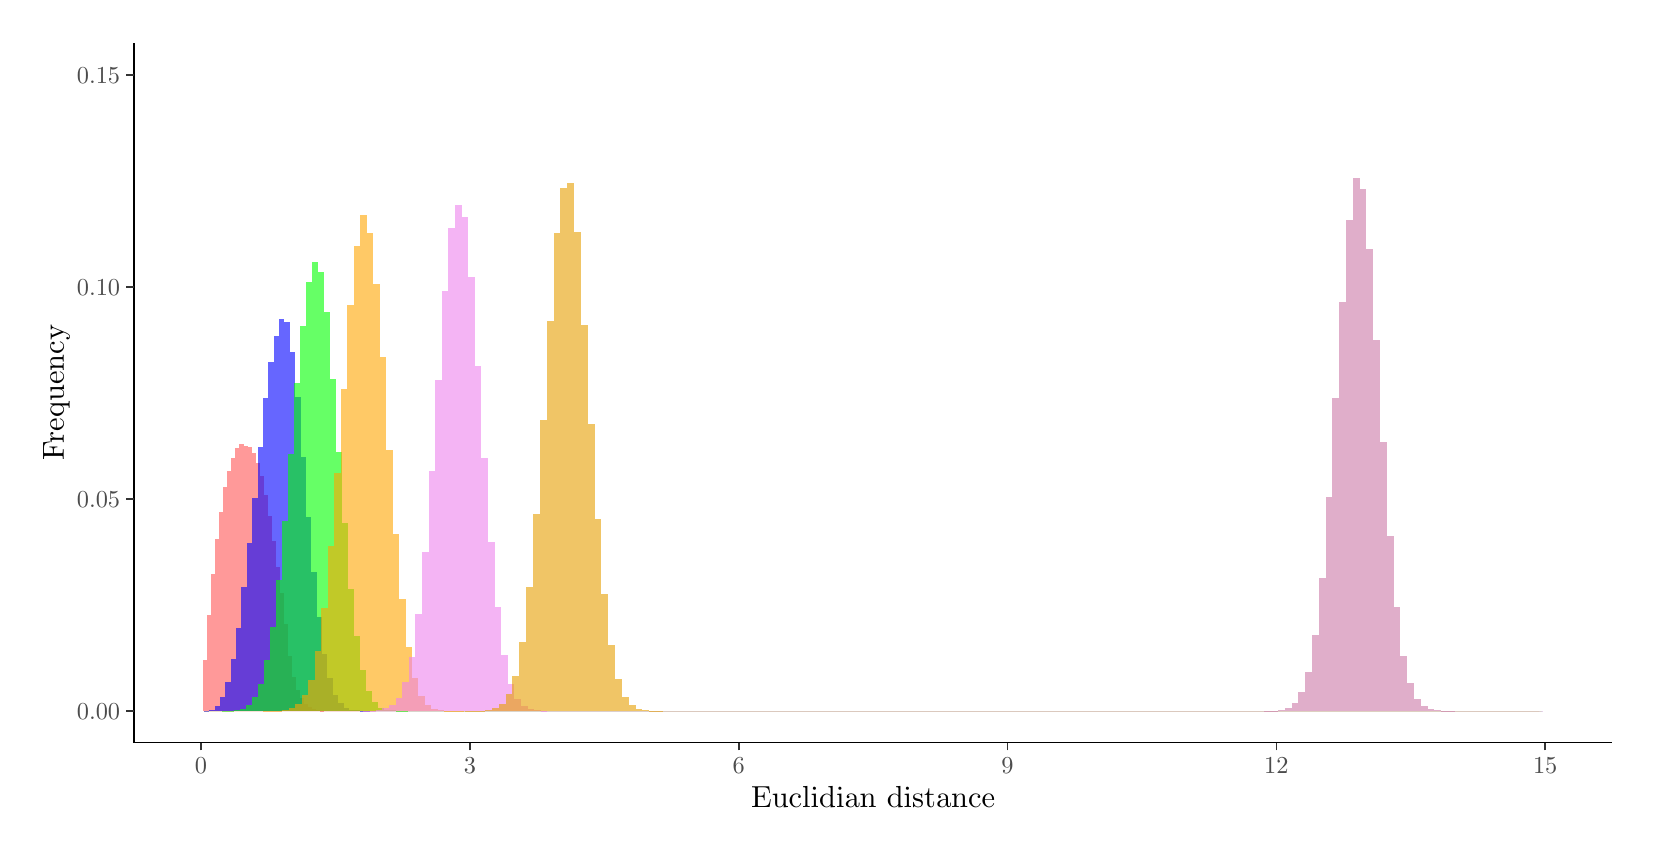
\begin{tikzpicture}[x=1pt,y=1pt]
\definecolor{fillColor}{RGB}{255,255,255}
\path[use as bounding box,fill=fillColor,fill opacity=0.00] (0,0) rectangle (578.16,289.08);
\begin{scope}
\path[clip] (  0.00,  0.00) rectangle (578.16,289.08);
\definecolor{drawColor}{RGB}{255,255,255}
\definecolor{fillColor}{RGB}{255,255,255}

\path[draw=drawColor,line width= 0.6pt,line join=round,line cap=round,fill=fillColor] (  0.00,  0.00) rectangle (578.16,289.08);
\end{scope}
\begin{scope}
\path[clip] ( 38.36, 30.72) rectangle (572.66,283.58);
\definecolor{fillColor}{RGB}{255,0,0}

\path[fill=fillColor,fill opacity=0.40] ( 63.38, 42.22) rectangle ( 64.84, 60.64);

\path[fill=fillColor,fill opacity=0.40] ( 64.84, 42.22) rectangle ( 66.30, 76.72);

\path[fill=fillColor,fill opacity=0.40] ( 66.30, 42.22) rectangle ( 67.76, 91.52);

\path[fill=fillColor,fill opacity=0.40] ( 67.76, 42.22) rectangle ( 69.23,104.41);

\path[fill=fillColor,fill opacity=0.40] ( 69.23, 42.22) rectangle ( 70.69,114.19);

\path[fill=fillColor,fill opacity=0.40] ( 70.69, 42.22) rectangle ( 72.15,123.13);

\path[fill=fillColor,fill opacity=0.40] ( 72.15, 42.22) rectangle ( 73.61,129.03);

\path[fill=fillColor,fill opacity=0.40] ( 73.61, 42.22) rectangle ( 75.08,133.45);

\path[fill=fillColor,fill opacity=0.40] ( 75.08, 42.22) rectangle ( 76.54,137.33);

\path[fill=fillColor,fill opacity=0.40] ( 76.54, 42.22) rectangle ( 78.00,138.66);

\path[fill=fillColor,fill opacity=0.40] ( 78.00, 42.22) rectangle ( 79.46,138.05);

\path[fill=fillColor,fill opacity=0.40] ( 79.46, 42.22) rectangle ( 80.93,137.39);

\path[fill=fillColor,fill opacity=0.40] ( 80.93, 42.22) rectangle ( 82.39,135.54);

\path[fill=fillColor,fill opacity=0.40] ( 82.39, 42.22) rectangle ( 83.85,131.75);

\path[fill=fillColor,fill opacity=0.40] ( 83.85, 42.22) rectangle ( 85.31,126.95);

\path[fill=fillColor,fill opacity=0.40] ( 85.31, 42.22) rectangle ( 86.77,120.10);

\path[fill=fillColor,fill opacity=0.40] ( 86.77, 42.22) rectangle ( 88.24,112.48);

\path[fill=fillColor,fill opacity=0.40] ( 88.24, 42.22) rectangle ( 89.70,103.49);

\path[fill=fillColor,fill opacity=0.40] ( 89.70, 42.22) rectangle ( 91.16, 94.31);

\path[fill=fillColor,fill opacity=0.40] ( 91.16, 42.22) rectangle ( 92.62, 84.84);

\path[fill=fillColor,fill opacity=0.40] ( 92.62, 42.22) rectangle ( 94.09, 73.51);

\path[fill=fillColor,fill opacity=0.40] ( 94.09, 42.22) rectangle ( 95.55, 62.03);

\path[fill=fillColor,fill opacity=0.40] ( 95.55, 42.22) rectangle ( 97.01, 54.55);

\path[fill=fillColor,fill opacity=0.40] ( 97.01, 42.22) rectangle ( 98.47, 49.92);

\path[fill=fillColor,fill opacity=0.40] ( 98.47, 42.22) rectangle ( 99.94, 46.82);

\path[fill=fillColor,fill opacity=0.40] ( 99.94, 42.22) rectangle (101.40, 44.75);

\path[fill=fillColor,fill opacity=0.40] (101.40, 42.22) rectangle (102.86, 43.56);

\path[fill=fillColor,fill opacity=0.40] (102.86, 42.22) rectangle (104.32, 42.75);

\path[fill=fillColor,fill opacity=0.40] (104.32, 42.22) rectangle (105.78, 42.40);

\path[fill=fillColor,fill opacity=0.40] (105.78, 42.22) rectangle (107.25, 42.23);

\path[fill=fillColor,fill opacity=0.40] (107.25, 42.22) rectangle (108.71, 42.22);

\path[fill=fillColor,fill opacity=0.40] (108.71, 42.22) rectangle (110.17, 42.22);

\path[fill=fillColor,fill opacity=0.40] (110.17, 42.22) rectangle (111.63, 42.22);

\path[fill=fillColor,fill opacity=0.40] (111.63, 42.22) rectangle (113.10, 42.22);

\path[fill=fillColor,fill opacity=0.40] (113.10, 42.22) rectangle (114.56, 42.22);

\path[fill=fillColor,fill opacity=0.40] (114.56, 42.22) rectangle (116.02, 42.22);

\path[fill=fillColor,fill opacity=0.40] (116.02, 42.22) rectangle (117.48, 42.22);

\path[fill=fillColor,fill opacity=0.40] (117.48, 42.22) rectangle (118.95, 42.22);

\path[fill=fillColor,fill opacity=0.40] (118.95, 42.22) rectangle (120.41, 42.22);

\path[fill=fillColor,fill opacity=0.40] (120.41, 42.22) rectangle (121.87, 42.22);

\path[fill=fillColor,fill opacity=0.40] (121.87, 42.22) rectangle (123.33, 42.22);

\path[fill=fillColor,fill opacity=0.40] (123.33, 42.22) rectangle (124.79, 42.22);

\path[fill=fillColor,fill opacity=0.40] (124.79, 42.22) rectangle (126.26, 42.22);

\path[fill=fillColor,fill opacity=0.40] (126.26, 42.22) rectangle (127.72, 42.22);

\path[fill=fillColor,fill opacity=0.40] (127.72, 42.22) rectangle (129.18, 42.22);

\path[fill=fillColor,fill opacity=0.40] (129.18, 42.22) rectangle (130.64, 42.22);

\path[fill=fillColor,fill opacity=0.40] (130.64, 42.22) rectangle (132.11, 42.22);

\path[fill=fillColor,fill opacity=0.40] (132.11, 42.22) rectangle (133.57, 42.22);

\path[fill=fillColor,fill opacity=0.40] (133.57, 42.22) rectangle (135.03, 42.22);

\path[fill=fillColor,fill opacity=0.40] (135.03, 42.22) rectangle (136.49, 42.22);

\path[fill=fillColor,fill opacity=0.40] (136.49, 42.22) rectangle (137.96, 42.22);

\path[fill=fillColor,fill opacity=0.40] (137.96, 42.22) rectangle (139.42, 42.22);

\path[fill=fillColor,fill opacity=0.40] (139.42, 42.22) rectangle (140.88, 42.22);

\path[fill=fillColor,fill opacity=0.40] (140.88, 42.22) rectangle (142.34, 42.22);

\path[fill=fillColor,fill opacity=0.40] (142.34, 42.22) rectangle (143.80, 42.22);

\path[fill=fillColor,fill opacity=0.40] (143.80, 42.22) rectangle (145.27, 42.22);

\path[fill=fillColor,fill opacity=0.40] (145.27, 42.22) rectangle (146.73, 42.22);

\path[fill=fillColor,fill opacity=0.40] (146.73, 42.22) rectangle (148.19, 42.22);

\path[fill=fillColor,fill opacity=0.40] (148.19, 42.22) rectangle (149.65, 42.22);

\path[fill=fillColor,fill opacity=0.40] (149.65, 42.22) rectangle (151.12, 42.22);

\path[fill=fillColor,fill opacity=0.40] (151.12, 42.22) rectangle (152.58, 42.22);

\path[fill=fillColor,fill opacity=0.40] (152.58, 42.22) rectangle (154.04, 42.22);

\path[fill=fillColor,fill opacity=0.40] (154.04, 42.22) rectangle (155.50, 42.22);

\path[fill=fillColor,fill opacity=0.40] (155.50, 42.22) rectangle (156.96, 42.22);

\path[fill=fillColor,fill opacity=0.40] (156.96, 42.22) rectangle (158.43, 42.22);

\path[fill=fillColor,fill opacity=0.40] (158.43, 42.22) rectangle (159.89, 42.22);

\path[fill=fillColor,fill opacity=0.40] (159.89, 42.22) rectangle (161.35, 42.22);

\path[fill=fillColor,fill opacity=0.40] (161.35, 42.22) rectangle (162.81, 42.22);

\path[fill=fillColor,fill opacity=0.40] (162.81, 42.22) rectangle (164.28, 42.22);

\path[fill=fillColor,fill opacity=0.40] (164.28, 42.22) rectangle (165.74, 42.22);

\path[fill=fillColor,fill opacity=0.40] (165.74, 42.22) rectangle (167.20, 42.22);

\path[fill=fillColor,fill opacity=0.40] (167.20, 42.22) rectangle (168.66, 42.22);

\path[fill=fillColor,fill opacity=0.40] (168.66, 42.22) rectangle (170.13, 42.22);

\path[fill=fillColor,fill opacity=0.40] (170.13, 42.22) rectangle (171.59, 42.22);

\path[fill=fillColor,fill opacity=0.40] (171.59, 42.22) rectangle (173.05, 42.22);

\path[fill=fillColor,fill opacity=0.40] (173.05, 42.22) rectangle (174.51, 42.22);

\path[fill=fillColor,fill opacity=0.40] (174.51, 42.22) rectangle (175.97, 42.22);

\path[fill=fillColor,fill opacity=0.40] (175.97, 42.22) rectangle (177.44, 42.22);

\path[fill=fillColor,fill opacity=0.40] (177.44, 42.22) rectangle (178.90, 42.22);

\path[fill=fillColor,fill opacity=0.40] (178.90, 42.22) rectangle (180.36, 42.22);

\path[fill=fillColor,fill opacity=0.40] (180.36, 42.22) rectangle (181.82, 42.22);

\path[fill=fillColor,fill opacity=0.40] (181.82, 42.22) rectangle (183.29, 42.22);

\path[fill=fillColor,fill opacity=0.40] (183.29, 42.22) rectangle (184.75, 42.22);

\path[fill=fillColor,fill opacity=0.40] (184.75, 42.22) rectangle (186.21, 42.22);

\path[fill=fillColor,fill opacity=0.40] (186.21, 42.22) rectangle (187.67, 42.22);

\path[fill=fillColor,fill opacity=0.40] (187.67, 42.22) rectangle (189.14, 42.22);

\path[fill=fillColor,fill opacity=0.40] (189.14, 42.22) rectangle (190.60, 42.22);

\path[fill=fillColor,fill opacity=0.40] (190.60, 42.22) rectangle (192.06, 42.22);

\path[fill=fillColor,fill opacity=0.40] (192.06, 42.22) rectangle (193.52, 42.22);

\path[fill=fillColor,fill opacity=0.40] (193.52, 42.22) rectangle (194.98, 42.22);

\path[fill=fillColor,fill opacity=0.40] (194.98, 42.22) rectangle (196.45, 42.22);

\path[fill=fillColor,fill opacity=0.40] (196.45, 42.22) rectangle (197.91, 42.22);

\path[fill=fillColor,fill opacity=0.40] (197.91, 42.22) rectangle (199.37, 42.22);

\path[fill=fillColor,fill opacity=0.40] (199.37, 42.22) rectangle (200.83, 42.22);

\path[fill=fillColor,fill opacity=0.40] (200.83, 42.22) rectangle (202.30, 42.22);

\path[fill=fillColor,fill opacity=0.40] (202.30, 42.22) rectangle (203.76, 42.22);

\path[fill=fillColor,fill opacity=0.40] (203.76, 42.22) rectangle (205.22, 42.22);

\path[fill=fillColor,fill opacity=0.40] (205.22, 42.22) rectangle (206.68, 42.22);

\path[fill=fillColor,fill opacity=0.40] (206.68, 42.22) rectangle (208.15, 42.22);

\path[fill=fillColor,fill opacity=0.40] (208.15, 42.22) rectangle (209.61, 42.22);

\path[fill=fillColor,fill opacity=0.40] (209.61, 42.22) rectangle (211.07, 42.22);

\path[fill=fillColor,fill opacity=0.40] (211.07, 42.22) rectangle (212.53, 42.22);

\path[fill=fillColor,fill opacity=0.40] (212.53, 42.22) rectangle (213.99, 42.22);

\path[fill=fillColor,fill opacity=0.40] (213.99, 42.22) rectangle (215.46, 42.22);

\path[fill=fillColor,fill opacity=0.40] (215.46, 42.22) rectangle (216.92, 42.22);

\path[fill=fillColor,fill opacity=0.40] (216.92, 42.22) rectangle (218.38, 42.22);

\path[fill=fillColor,fill opacity=0.40] (218.38, 42.22) rectangle (219.84, 42.22);

\path[fill=fillColor,fill opacity=0.40] (219.84, 42.22) rectangle (221.31, 42.22);

\path[fill=fillColor,fill opacity=0.40] (221.31, 42.22) rectangle (222.77, 42.22);

\path[fill=fillColor,fill opacity=0.40] (222.77, 42.22) rectangle (224.23, 42.22);

\path[fill=fillColor,fill opacity=0.40] (224.23, 42.22) rectangle (225.69, 42.22);

\path[fill=fillColor,fill opacity=0.40] (225.69, 42.22) rectangle (227.16, 42.22);

\path[fill=fillColor,fill opacity=0.40] (227.16, 42.22) rectangle (228.62, 42.22);

\path[fill=fillColor,fill opacity=0.40] (228.62, 42.22) rectangle (230.08, 42.22);

\path[fill=fillColor,fill opacity=0.40] (230.08, 42.22) rectangle (231.54, 42.22);

\path[fill=fillColor,fill opacity=0.40] (231.54, 42.22) rectangle (233.00, 42.22);

\path[fill=fillColor,fill opacity=0.40] (233.00, 42.22) rectangle (234.47, 42.22);

\path[fill=fillColor,fill opacity=0.40] (234.47, 42.22) rectangle (235.93, 42.22);

\path[fill=fillColor,fill opacity=0.40] (235.93, 42.22) rectangle (237.39, 42.22);

\path[fill=fillColor,fill opacity=0.40] (237.39, 42.22) rectangle (238.85, 42.22);

\path[fill=fillColor,fill opacity=0.40] (238.85, 42.22) rectangle (240.32, 42.22);

\path[fill=fillColor,fill opacity=0.40] (240.32, 42.22) rectangle (241.78, 42.22);

\path[fill=fillColor,fill opacity=0.40] (241.78, 42.22) rectangle (243.24, 42.22);

\path[fill=fillColor,fill opacity=0.40] (243.24, 42.22) rectangle (244.70, 42.22);

\path[fill=fillColor,fill opacity=0.40] (244.70, 42.22) rectangle (246.16, 42.22);

\path[fill=fillColor,fill opacity=0.40] (246.16, 42.22) rectangle (247.63, 42.22);

\path[fill=fillColor,fill opacity=0.40] (247.63, 42.22) rectangle (249.09, 42.22);

\path[fill=fillColor,fill opacity=0.40] (249.09, 42.22) rectangle (250.55, 42.22);

\path[fill=fillColor,fill opacity=0.40] (250.55, 42.22) rectangle (252.01, 42.22);

\path[fill=fillColor,fill opacity=0.40] (252.01, 42.22) rectangle (253.48, 42.22);

\path[fill=fillColor,fill opacity=0.40] (253.48, 42.22) rectangle (254.94, 42.22);

\path[fill=fillColor,fill opacity=0.40] (254.94, 42.22) rectangle (256.40, 42.22);

\path[fill=fillColor,fill opacity=0.40] (256.40, 42.22) rectangle (257.86, 42.22);

\path[fill=fillColor,fill opacity=0.40] (257.86, 42.22) rectangle (259.33, 42.22);

\path[fill=fillColor,fill opacity=0.40] (259.33, 42.22) rectangle (260.79, 42.22);

\path[fill=fillColor,fill opacity=0.40] (260.79, 42.22) rectangle (262.25, 42.22);

\path[fill=fillColor,fill opacity=0.40] (262.25, 42.22) rectangle (263.71, 42.22);

\path[fill=fillColor,fill opacity=0.40] (263.71, 42.22) rectangle (265.17, 42.22);

\path[fill=fillColor,fill opacity=0.40] (265.17, 42.22) rectangle (266.64, 42.22);

\path[fill=fillColor,fill opacity=0.40] (266.64, 42.22) rectangle (268.10, 42.22);

\path[fill=fillColor,fill opacity=0.40] (268.10, 42.22) rectangle (269.56, 42.22);

\path[fill=fillColor,fill opacity=0.40] (269.56, 42.22) rectangle (271.02, 42.22);

\path[fill=fillColor,fill opacity=0.40] (271.02, 42.22) rectangle (272.49, 42.22);

\path[fill=fillColor,fill opacity=0.40] (272.49, 42.22) rectangle (273.95, 42.22);

\path[fill=fillColor,fill opacity=0.40] (273.95, 42.22) rectangle (275.41, 42.22);

\path[fill=fillColor,fill opacity=0.40] (275.41, 42.22) rectangle (276.87, 42.22);

\path[fill=fillColor,fill opacity=0.40] (276.87, 42.22) rectangle (278.34, 42.22);

\path[fill=fillColor,fill opacity=0.40] (278.34, 42.22) rectangle (279.80, 42.22);

\path[fill=fillColor,fill opacity=0.40] (279.80, 42.22) rectangle (281.26, 42.22);

\path[fill=fillColor,fill opacity=0.40] (281.26, 42.22) rectangle (282.72, 42.22);

\path[fill=fillColor,fill opacity=0.40] (282.72, 42.22) rectangle (284.18, 42.22);

\path[fill=fillColor,fill opacity=0.40] (284.18, 42.22) rectangle (285.65, 42.22);

\path[fill=fillColor,fill opacity=0.40] (285.65, 42.22) rectangle (287.11, 42.22);

\path[fill=fillColor,fill opacity=0.40] (287.11, 42.22) rectangle (288.57, 42.22);

\path[fill=fillColor,fill opacity=0.40] (288.57, 42.22) rectangle (290.03, 42.22);

\path[fill=fillColor,fill opacity=0.40] (290.03, 42.22) rectangle (291.50, 42.22);

\path[fill=fillColor,fill opacity=0.40] (291.50, 42.22) rectangle (292.96, 42.22);

\path[fill=fillColor,fill opacity=0.40] (292.96, 42.22) rectangle (294.42, 42.22);

\path[fill=fillColor,fill opacity=0.40] (294.42, 42.22) rectangle (295.88, 42.22);

\path[fill=fillColor,fill opacity=0.40] (295.88, 42.22) rectangle (297.35, 42.22);

\path[fill=fillColor,fill opacity=0.40] (297.35, 42.22) rectangle (298.81, 42.22);

\path[fill=fillColor,fill opacity=0.40] (298.81, 42.22) rectangle (300.27, 42.22);

\path[fill=fillColor,fill opacity=0.40] (300.27, 42.22) rectangle (301.73, 42.22);

\path[fill=fillColor,fill opacity=0.40] (301.73, 42.22) rectangle (303.19, 42.22);

\path[fill=fillColor,fill opacity=0.40] (303.19, 42.22) rectangle (304.66, 42.22);

\path[fill=fillColor,fill opacity=0.40] (304.66, 42.22) rectangle (306.12, 42.22);

\path[fill=fillColor,fill opacity=0.40] (306.12, 42.22) rectangle (307.58, 42.22);

\path[fill=fillColor,fill opacity=0.40] (307.58, 42.22) rectangle (309.04, 42.22);

\path[fill=fillColor,fill opacity=0.40] (309.04, 42.22) rectangle (310.51, 42.22);

\path[fill=fillColor,fill opacity=0.40] (310.51, 42.22) rectangle (311.97, 42.22);

\path[fill=fillColor,fill opacity=0.40] (311.97, 42.22) rectangle (313.43, 42.22);

\path[fill=fillColor,fill opacity=0.40] (313.43, 42.22) rectangle (314.89, 42.22);

\path[fill=fillColor,fill opacity=0.40] (314.89, 42.22) rectangle (316.36, 42.22);

\path[fill=fillColor,fill opacity=0.40] (316.36, 42.22) rectangle (317.82, 42.22);

\path[fill=fillColor,fill opacity=0.40] (317.82, 42.22) rectangle (319.28, 42.22);

\path[fill=fillColor,fill opacity=0.40] (319.28, 42.22) rectangle (320.74, 42.22);

\path[fill=fillColor,fill opacity=0.40] (320.74, 42.22) rectangle (322.20, 42.22);

\path[fill=fillColor,fill opacity=0.40] (322.20, 42.22) rectangle (323.67, 42.22);

\path[fill=fillColor,fill opacity=0.40] (323.67, 42.22) rectangle (325.13, 42.22);

\path[fill=fillColor,fill opacity=0.40] (325.13, 42.22) rectangle (326.59, 42.22);

\path[fill=fillColor,fill opacity=0.40] (326.59, 42.22) rectangle (328.05, 42.22);

\path[fill=fillColor,fill opacity=0.40] (328.05, 42.22) rectangle (329.52, 42.22);

\path[fill=fillColor,fill opacity=0.40] (329.52, 42.22) rectangle (330.98, 42.22);

\path[fill=fillColor,fill opacity=0.40] (330.98, 42.22) rectangle (332.44, 42.22);

\path[fill=fillColor,fill opacity=0.40] (332.44, 42.22) rectangle (333.90, 42.22);

\path[fill=fillColor,fill opacity=0.40] (333.90, 42.22) rectangle (335.36, 42.22);

\path[fill=fillColor,fill opacity=0.40] (335.36, 42.22) rectangle (336.83, 42.22);

\path[fill=fillColor,fill opacity=0.40] (336.83, 42.22) rectangle (338.29, 42.22);

\path[fill=fillColor,fill opacity=0.40] (338.29, 42.22) rectangle (339.75, 42.22);

\path[fill=fillColor,fill opacity=0.40] (339.75, 42.22) rectangle (341.21, 42.22);

\path[fill=fillColor,fill opacity=0.40] (341.21, 42.22) rectangle (342.68, 42.22);

\path[fill=fillColor,fill opacity=0.40] (342.68, 42.22) rectangle (344.14, 42.22);

\path[fill=fillColor,fill opacity=0.40] (344.14, 42.22) rectangle (345.60, 42.22);

\path[fill=fillColor,fill opacity=0.40] (345.60, 42.22) rectangle (347.06, 42.22);

\path[fill=fillColor,fill opacity=0.40] (347.06, 42.22) rectangle (348.53, 42.22);

\path[fill=fillColor,fill opacity=0.40] (348.53, 42.22) rectangle (349.99, 42.22);

\path[fill=fillColor,fill opacity=0.40] (349.99, 42.22) rectangle (351.45, 42.22);

\path[fill=fillColor,fill opacity=0.40] (351.45, 42.22) rectangle (352.91, 42.22);

\path[fill=fillColor,fill opacity=0.40] (352.91, 42.22) rectangle (354.37, 42.22);

\path[fill=fillColor,fill opacity=0.40] (354.37, 42.22) rectangle (355.84, 42.22);

\path[fill=fillColor,fill opacity=0.40] (355.84, 42.22) rectangle (357.30, 42.22);

\path[fill=fillColor,fill opacity=0.40] (357.30, 42.22) rectangle (358.76, 42.22);

\path[fill=fillColor,fill opacity=0.40] (358.76, 42.22) rectangle (360.22, 42.22);

\path[fill=fillColor,fill opacity=0.40] (360.22, 42.22) rectangle (361.69, 42.22);

\path[fill=fillColor,fill opacity=0.40] (361.69, 42.22) rectangle (363.15, 42.22);

\path[fill=fillColor,fill opacity=0.40] (363.15, 42.22) rectangle (364.61, 42.22);

\path[fill=fillColor,fill opacity=0.40] (364.61, 42.22) rectangle (366.07, 42.22);

\path[fill=fillColor,fill opacity=0.40] (366.07, 42.22) rectangle (367.54, 42.22);

\path[fill=fillColor,fill opacity=0.40] (367.54, 42.22) rectangle (369.00, 42.22);

\path[fill=fillColor,fill opacity=0.40] (369.00, 42.22) rectangle (370.46, 42.22);

\path[fill=fillColor,fill opacity=0.40] (370.46, 42.22) rectangle (371.92, 42.22);

\path[fill=fillColor,fill opacity=0.40] (371.92, 42.22) rectangle (373.38, 42.22);

\path[fill=fillColor,fill opacity=0.40] (373.38, 42.22) rectangle (374.85, 42.22);

\path[fill=fillColor,fill opacity=0.40] (374.85, 42.22) rectangle (376.31, 42.22);

\path[fill=fillColor,fill opacity=0.40] (376.31, 42.22) rectangle (377.77, 42.22);

\path[fill=fillColor,fill opacity=0.40] (377.77, 42.22) rectangle (379.23, 42.22);

\path[fill=fillColor,fill opacity=0.40] (379.23, 42.22) rectangle (380.70, 42.22);

\path[fill=fillColor,fill opacity=0.40] (380.70, 42.22) rectangle (382.16, 42.22);

\path[fill=fillColor,fill opacity=0.40] (382.16, 42.22) rectangle (383.62, 42.22);

\path[fill=fillColor,fill opacity=0.40] (383.62, 42.22) rectangle (385.08, 42.22);

\path[fill=fillColor,fill opacity=0.40] (385.08, 42.22) rectangle (386.55, 42.22);

\path[fill=fillColor,fill opacity=0.40] (386.55, 42.22) rectangle (388.01, 42.22);

\path[fill=fillColor,fill opacity=0.40] (388.01, 42.22) rectangle (389.47, 42.22);

\path[fill=fillColor,fill opacity=0.40] (389.47, 42.22) rectangle (390.93, 42.22);

\path[fill=fillColor,fill opacity=0.40] (390.93, 42.22) rectangle (392.39, 42.22);

\path[fill=fillColor,fill opacity=0.40] (392.39, 42.22) rectangle (393.86, 42.22);

\path[fill=fillColor,fill opacity=0.40] (393.86, 42.22) rectangle (395.32, 42.22);

\path[fill=fillColor,fill opacity=0.40] (395.32, 42.22) rectangle (396.78, 42.22);

\path[fill=fillColor,fill opacity=0.40] (396.78, 42.22) rectangle (398.24, 42.22);

\path[fill=fillColor,fill opacity=0.40] (398.24, 42.22) rectangle (399.71, 42.22);

\path[fill=fillColor,fill opacity=0.40] (399.71, 42.22) rectangle (401.17, 42.22);

\path[fill=fillColor,fill opacity=0.40] (401.17, 42.22) rectangle (402.63, 42.22);

\path[fill=fillColor,fill opacity=0.40] (402.63, 42.22) rectangle (404.09, 42.22);

\path[fill=fillColor,fill opacity=0.40] (404.09, 42.22) rectangle (405.56, 42.22);

\path[fill=fillColor,fill opacity=0.40] (405.56, 42.22) rectangle (407.02, 42.22);

\path[fill=fillColor,fill opacity=0.40] (407.02, 42.22) rectangle (408.48, 42.22);

\path[fill=fillColor,fill opacity=0.40] (408.48, 42.22) rectangle (409.94, 42.22);

\path[fill=fillColor,fill opacity=0.40] (409.94, 42.22) rectangle (411.40, 42.22);

\path[fill=fillColor,fill opacity=0.40] (411.40, 42.22) rectangle (412.87, 42.22);

\path[fill=fillColor,fill opacity=0.40] (412.87, 42.22) rectangle (414.33, 42.22);

\path[fill=fillColor,fill opacity=0.40] (414.33, 42.22) rectangle (415.79, 42.22);

\path[fill=fillColor,fill opacity=0.40] (415.79, 42.22) rectangle (417.25, 42.22);

\path[fill=fillColor,fill opacity=0.40] (417.25, 42.22) rectangle (418.72, 42.22);

\path[fill=fillColor,fill opacity=0.40] (418.72, 42.22) rectangle (420.18, 42.22);

\path[fill=fillColor,fill opacity=0.40] (420.18, 42.22) rectangle (421.64, 42.22);

\path[fill=fillColor,fill opacity=0.40] (421.64, 42.22) rectangle (423.10, 42.22);

\path[fill=fillColor,fill opacity=0.40] (423.10, 42.22) rectangle (424.56, 42.22);

\path[fill=fillColor,fill opacity=0.40] (424.56, 42.22) rectangle (426.03, 42.22);

\path[fill=fillColor,fill opacity=0.40] (426.03, 42.22) rectangle (427.49, 42.22);

\path[fill=fillColor,fill opacity=0.40] (427.49, 42.22) rectangle (428.95, 42.22);

\path[fill=fillColor,fill opacity=0.40] (428.95, 42.22) rectangle (430.41, 42.22);

\path[fill=fillColor,fill opacity=0.40] (430.41, 42.22) rectangle (431.88, 42.22);

\path[fill=fillColor,fill opacity=0.40] (431.88, 42.22) rectangle (433.34, 42.22);

\path[fill=fillColor,fill opacity=0.40] (433.34, 42.22) rectangle (434.80, 42.22);

\path[fill=fillColor,fill opacity=0.40] (434.80, 42.22) rectangle (436.26, 42.22);

\path[fill=fillColor,fill opacity=0.40] (436.26, 42.22) rectangle (437.73, 42.22);

\path[fill=fillColor,fill opacity=0.40] (437.73, 42.22) rectangle (439.19, 42.22);

\path[fill=fillColor,fill opacity=0.40] (439.19, 42.22) rectangle (440.65, 42.22);

\path[fill=fillColor,fill opacity=0.40] (440.65, 42.22) rectangle (442.11, 42.22);

\path[fill=fillColor,fill opacity=0.40] (442.11, 42.22) rectangle (443.57, 42.22);

\path[fill=fillColor,fill opacity=0.40] (443.57, 42.22) rectangle (445.04, 42.22);

\path[fill=fillColor,fill opacity=0.40] (445.04, 42.22) rectangle (446.50, 42.22);

\path[fill=fillColor,fill opacity=0.40] (446.50, 42.22) rectangle (447.96, 42.22);

\path[fill=fillColor,fill opacity=0.40] (447.96, 42.22) rectangle (449.42, 42.22);

\path[fill=fillColor,fill opacity=0.40] (449.42, 42.22) rectangle (450.89, 42.22);

\path[fill=fillColor,fill opacity=0.40] (450.89, 42.22) rectangle (452.35, 42.22);

\path[fill=fillColor,fill opacity=0.40] (452.35, 42.22) rectangle (453.81, 42.22);

\path[fill=fillColor,fill opacity=0.40] (453.81, 42.22) rectangle (455.27, 42.22);

\path[fill=fillColor,fill opacity=0.40] (455.27, 42.22) rectangle (456.74, 42.22);

\path[fill=fillColor,fill opacity=0.40] (456.74, 42.22) rectangle (458.20, 42.22);

\path[fill=fillColor,fill opacity=0.40] (458.20, 42.22) rectangle (459.66, 42.22);

\path[fill=fillColor,fill opacity=0.40] (459.66, 42.22) rectangle (461.12, 42.22);

\path[fill=fillColor,fill opacity=0.40] (461.12, 42.22) rectangle (462.58, 42.22);

\path[fill=fillColor,fill opacity=0.40] (462.58, 42.22) rectangle (464.05, 42.22);

\path[fill=fillColor,fill opacity=0.40] (464.05, 42.22) rectangle (465.51, 42.22);

\path[fill=fillColor,fill opacity=0.40] (465.51, 42.22) rectangle (466.97, 42.22);

\path[fill=fillColor,fill opacity=0.40] (466.97, 42.22) rectangle (468.43, 42.22);

\path[fill=fillColor,fill opacity=0.40] (468.43, 42.22) rectangle (469.90, 42.22);

\path[fill=fillColor,fill opacity=0.40] (469.90, 42.22) rectangle (471.36, 42.22);

\path[fill=fillColor,fill opacity=0.40] (471.36, 42.22) rectangle (472.82, 42.22);

\path[fill=fillColor,fill opacity=0.40] (472.82, 42.22) rectangle (474.28, 42.22);

\path[fill=fillColor,fill opacity=0.40] (474.28, 42.22) rectangle (475.75, 42.22);

\path[fill=fillColor,fill opacity=0.40] (475.75, 42.22) rectangle (477.21, 42.22);

\path[fill=fillColor,fill opacity=0.40] (477.21, 42.22) rectangle (478.67, 42.22);

\path[fill=fillColor,fill opacity=0.40] (478.67, 42.22) rectangle (480.13, 42.22);

\path[fill=fillColor,fill opacity=0.40] (480.13, 42.22) rectangle (481.59, 42.22);

\path[fill=fillColor,fill opacity=0.40] (481.59, 42.22) rectangle (483.06, 42.22);

\path[fill=fillColor,fill opacity=0.40] (483.06, 42.22) rectangle (484.52, 42.22);

\path[fill=fillColor,fill opacity=0.40] (484.52, 42.22) rectangle (485.98, 42.22);

\path[fill=fillColor,fill opacity=0.40] (485.98, 42.22) rectangle (487.44, 42.22);

\path[fill=fillColor,fill opacity=0.40] (487.44, 42.22) rectangle (488.91, 42.22);

\path[fill=fillColor,fill opacity=0.40] (488.91, 42.22) rectangle (490.37, 42.22);

\path[fill=fillColor,fill opacity=0.40] (490.37, 42.22) rectangle (491.83, 42.22);

\path[fill=fillColor,fill opacity=0.40] (491.83, 42.22) rectangle (493.29, 42.22);

\path[fill=fillColor,fill opacity=0.40] (493.29, 42.22) rectangle (494.76, 42.22);

\path[fill=fillColor,fill opacity=0.40] (494.76, 42.22) rectangle (496.22, 42.22);

\path[fill=fillColor,fill opacity=0.40] (496.22, 42.22) rectangle (497.68, 42.22);

\path[fill=fillColor,fill opacity=0.40] (497.68, 42.22) rectangle (499.14, 42.22);

\path[fill=fillColor,fill opacity=0.40] (499.14, 42.22) rectangle (500.60, 42.22);

\path[fill=fillColor,fill opacity=0.40] (500.60, 42.22) rectangle (502.07, 42.22);

\path[fill=fillColor,fill opacity=0.40] (502.07, 42.22) rectangle (503.53, 42.22);

\path[fill=fillColor,fill opacity=0.40] (503.53, 42.22) rectangle (504.99, 42.22);

\path[fill=fillColor,fill opacity=0.40] (504.99, 42.22) rectangle (506.45, 42.22);

\path[fill=fillColor,fill opacity=0.40] (506.45, 42.22) rectangle (507.92, 42.22);

\path[fill=fillColor,fill opacity=0.40] (507.92, 42.22) rectangle (509.38, 42.22);

\path[fill=fillColor,fill opacity=0.40] (509.38, 42.22) rectangle (510.84, 42.22);

\path[fill=fillColor,fill opacity=0.40] (510.84, 42.22) rectangle (512.30, 42.22);

\path[fill=fillColor,fill opacity=0.40] (512.30, 42.22) rectangle (513.76, 42.22);

\path[fill=fillColor,fill opacity=0.40] (513.76, 42.22) rectangle (515.23, 42.22);

\path[fill=fillColor,fill opacity=0.40] (515.23, 42.22) rectangle (516.69, 42.22);

\path[fill=fillColor,fill opacity=0.40] (516.69, 42.22) rectangle (518.15, 42.22);

\path[fill=fillColor,fill opacity=0.40] (518.15, 42.22) rectangle (519.61, 42.22);

\path[fill=fillColor,fill opacity=0.40] (519.61, 42.22) rectangle (521.08, 42.22);

\path[fill=fillColor,fill opacity=0.40] (521.08, 42.22) rectangle (522.54, 42.22);

\path[fill=fillColor,fill opacity=0.40] (522.54, 42.22) rectangle (524.00, 42.22);

\path[fill=fillColor,fill opacity=0.40] (524.00, 42.22) rectangle (525.46, 42.22);

\path[fill=fillColor,fill opacity=0.40] (525.46, 42.22) rectangle (526.93, 42.22);

\path[fill=fillColor,fill opacity=0.40] (526.93, 42.22) rectangle (528.39, 42.22);

\path[fill=fillColor,fill opacity=0.40] (528.39, 42.22) rectangle (529.85, 42.22);

\path[fill=fillColor,fill opacity=0.40] (529.85, 42.22) rectangle (531.31, 42.22);

\path[fill=fillColor,fill opacity=0.40] (531.31, 42.22) rectangle (532.77, 42.22);

\path[fill=fillColor,fill opacity=0.40] (532.77, 42.22) rectangle (534.24, 42.22);

\path[fill=fillColor,fill opacity=0.40] (534.24, 42.22) rectangle (535.70, 42.22);

\path[fill=fillColor,fill opacity=0.40] (535.70, 42.22) rectangle (537.16, 42.22);

\path[fill=fillColor,fill opacity=0.40] (537.16, 42.22) rectangle (538.62, 42.22);

\path[fill=fillColor,fill opacity=0.40] (538.62, 42.22) rectangle (540.09, 42.22);

\path[fill=fillColor,fill opacity=0.40] (540.09, 42.22) rectangle (541.55, 42.22);

\path[fill=fillColor,fill opacity=0.40] (541.55, 42.22) rectangle (543.01, 42.22);

\path[fill=fillColor,fill opacity=0.40] (543.01, 42.22) rectangle (544.47, 42.22);

\path[fill=fillColor,fill opacity=0.40] (544.47, 42.22) rectangle (545.94, 42.22);

\path[fill=fillColor,fill opacity=0.40] (545.94, 42.22) rectangle (547.40, 42.22);
\definecolor{fillColor}{RGB}{0,0,255}

\path[fill=fillColor,fill opacity=0.60] ( 63.62, 42.22) rectangle ( 65.56, 42.25);

\path[fill=fillColor,fill opacity=0.60] ( 65.56, 42.22) rectangle ( 67.51, 42.69);

\path[fill=fillColor,fill opacity=0.60] ( 67.51, 42.22) rectangle ( 69.45, 43.96);

\path[fill=fillColor,fill opacity=0.60] ( 69.45, 42.22) rectangle ( 71.39, 47.07);

\path[fill=fillColor,fill opacity=0.60] ( 71.39, 42.22) rectangle ( 73.34, 52.70);

\path[fill=fillColor,fill opacity=0.60] ( 73.34, 42.22) rectangle ( 75.28, 61.08);

\path[fill=fillColor,fill opacity=0.60] ( 75.28, 42.22) rectangle ( 77.22, 72.06);

\path[fill=fillColor,fill opacity=0.60] ( 77.22, 42.22) rectangle ( 79.17, 86.95);

\path[fill=fillColor,fill opacity=0.60] ( 79.17, 42.22) rectangle ( 81.11,103.04);

\path[fill=fillColor,fill opacity=0.60] ( 81.11, 42.22) rectangle ( 83.05,119.22);

\path[fill=fillColor,fill opacity=0.60] ( 83.05, 42.22) rectangle ( 85.00,137.44);

\path[fill=fillColor,fill opacity=0.60] ( 85.00, 42.22) rectangle ( 86.94,155.14);

\path[fill=fillColor,fill opacity=0.60] ( 86.94, 42.22) rectangle ( 88.88,168.20);

\path[fill=fillColor,fill opacity=0.60] ( 88.88, 42.22) rectangle ( 90.83,177.50);

\path[fill=fillColor,fill opacity=0.60] ( 90.83, 42.22) rectangle ( 92.77,183.87);

\path[fill=fillColor,fill opacity=0.60] ( 92.77, 42.22) rectangle ( 94.72,182.87);

\path[fill=fillColor,fill opacity=0.60] ( 94.72, 42.22) rectangle ( 96.66,171.82);

\path[fill=fillColor,fill opacity=0.60] ( 96.66, 42.22) rectangle ( 98.60,155.45);

\path[fill=fillColor,fill opacity=0.60] ( 98.60, 42.22) rectangle (100.55,133.79);

\path[fill=fillColor,fill opacity=0.60] (100.55, 42.22) rectangle (102.49,112.34);

\path[fill=fillColor,fill opacity=0.60] (102.49, 42.22) rectangle (104.43, 92.47);

\path[fill=fillColor,fill opacity=0.60] (104.43, 42.22) rectangle (106.38, 76.30);

\path[fill=fillColor,fill opacity=0.60] (106.38, 42.22) rectangle (108.32, 62.80);

\path[fill=fillColor,fill opacity=0.60] (108.32, 42.22) rectangle (110.26, 54.20);

\path[fill=fillColor,fill opacity=0.60] (110.26, 42.22) rectangle (112.21, 48.03);

\path[fill=fillColor,fill opacity=0.60] (112.21, 42.22) rectangle (114.15, 45.05);

\path[fill=fillColor,fill opacity=0.60] (114.15, 42.22) rectangle (116.09, 43.40);

\path[fill=fillColor,fill opacity=0.60] (116.09, 42.22) rectangle (118.04, 42.67);

\path[fill=fillColor,fill opacity=0.60] (118.04, 42.22) rectangle (119.98, 42.36);

\path[fill=fillColor,fill opacity=0.60] (119.98, 42.22) rectangle (121.92, 42.25);

\path[fill=fillColor,fill opacity=0.60] (121.92, 42.22) rectangle (123.87, 42.23);

\path[fill=fillColor,fill opacity=0.60] (123.87, 42.22) rectangle (125.81, 42.22);

\path[fill=fillColor,fill opacity=0.60] (125.81, 42.22) rectangle (127.76, 42.22);

\path[fill=fillColor,fill opacity=0.60] (127.76, 42.22) rectangle (129.70, 42.22);

\path[fill=fillColor,fill opacity=0.60] (129.70, 42.22) rectangle (131.64, 42.22);

\path[fill=fillColor,fill opacity=0.60] (131.64, 42.22) rectangle (133.59, 42.22);

\path[fill=fillColor,fill opacity=0.60] (133.59, 42.22) rectangle (135.53, 42.22);

\path[fill=fillColor,fill opacity=0.60] (135.53, 42.22) rectangle (137.47, 42.22);

\path[fill=fillColor,fill opacity=0.60] (137.47, 42.22) rectangle (139.42, 42.22);

\path[fill=fillColor,fill opacity=0.60] (139.42, 42.22) rectangle (141.36, 42.22);

\path[fill=fillColor,fill opacity=0.60] (141.36, 42.22) rectangle (143.30, 42.22);

\path[fill=fillColor,fill opacity=0.60] (143.30, 42.22) rectangle (145.25, 42.22);

\path[fill=fillColor,fill opacity=0.60] (145.25, 42.22) rectangle (147.19, 42.22);

\path[fill=fillColor,fill opacity=0.60] (147.19, 42.22) rectangle (149.13, 42.22);

\path[fill=fillColor,fill opacity=0.60] (149.13, 42.22) rectangle (151.08, 42.22);

\path[fill=fillColor,fill opacity=0.60] (151.08, 42.22) rectangle (153.02, 42.22);

\path[fill=fillColor,fill opacity=0.60] (153.02, 42.22) rectangle (154.96, 42.22);

\path[fill=fillColor,fill opacity=0.60] (154.96, 42.22) rectangle (156.91, 42.22);

\path[fill=fillColor,fill opacity=0.60] (156.91, 42.22) rectangle (158.85, 42.22);

\path[fill=fillColor,fill opacity=0.60] (158.85, 42.22) rectangle (160.80, 42.22);

\path[fill=fillColor,fill opacity=0.60] (160.80, 42.22) rectangle (162.74, 42.22);

\path[fill=fillColor,fill opacity=0.60] (162.74, 42.22) rectangle (164.68, 42.22);

\path[fill=fillColor,fill opacity=0.60] (164.68, 42.22) rectangle (166.63, 42.22);

\path[fill=fillColor,fill opacity=0.60] (166.63, 42.22) rectangle (168.57, 42.22);

\path[fill=fillColor,fill opacity=0.60] (168.57, 42.22) rectangle (170.51, 42.22);

\path[fill=fillColor,fill opacity=0.60] (170.51, 42.22) rectangle (172.46, 42.22);

\path[fill=fillColor,fill opacity=0.60] (172.46, 42.22) rectangle (174.40, 42.22);

\path[fill=fillColor,fill opacity=0.60] (174.40, 42.22) rectangle (176.34, 42.22);

\path[fill=fillColor,fill opacity=0.60] (176.34, 42.22) rectangle (178.29, 42.22);

\path[fill=fillColor,fill opacity=0.60] (178.29, 42.22) rectangle (180.23, 42.22);

\path[fill=fillColor,fill opacity=0.60] (180.23, 42.22) rectangle (182.17, 42.22);

\path[fill=fillColor,fill opacity=0.60] (182.17, 42.22) rectangle (184.12, 42.22);

\path[fill=fillColor,fill opacity=0.60] (184.12, 42.22) rectangle (186.06, 42.22);

\path[fill=fillColor,fill opacity=0.60] (186.06, 42.22) rectangle (188.00, 42.22);

\path[fill=fillColor,fill opacity=0.60] (188.00, 42.22) rectangle (189.95, 42.22);

\path[fill=fillColor,fill opacity=0.60] (189.95, 42.22) rectangle (191.89, 42.22);

\path[fill=fillColor,fill opacity=0.60] (191.89, 42.22) rectangle (193.84, 42.22);

\path[fill=fillColor,fill opacity=0.60] (193.84, 42.22) rectangle (195.78, 42.22);

\path[fill=fillColor,fill opacity=0.60] (195.78, 42.22) rectangle (197.72, 42.22);

\path[fill=fillColor,fill opacity=0.60] (197.72, 42.22) rectangle (199.67, 42.22);

\path[fill=fillColor,fill opacity=0.60] (199.67, 42.22) rectangle (201.61, 42.22);

\path[fill=fillColor,fill opacity=0.60] (201.61, 42.22) rectangle (203.55, 42.22);

\path[fill=fillColor,fill opacity=0.60] (203.55, 42.22) rectangle (205.50, 42.22);

\path[fill=fillColor,fill opacity=0.60] (205.50, 42.22) rectangle (207.44, 42.22);

\path[fill=fillColor,fill opacity=0.60] (207.44, 42.22) rectangle (209.38, 42.22);

\path[fill=fillColor,fill opacity=0.60] (209.38, 42.22) rectangle (211.33, 42.22);

\path[fill=fillColor,fill opacity=0.60] (211.33, 42.22) rectangle (213.27, 42.22);

\path[fill=fillColor,fill opacity=0.60] (213.27, 42.22) rectangle (215.21, 42.22);

\path[fill=fillColor,fill opacity=0.60] (215.21, 42.22) rectangle (217.16, 42.22);

\path[fill=fillColor,fill opacity=0.60] (217.16, 42.22) rectangle (219.10, 42.22);

\path[fill=fillColor,fill opacity=0.60] (219.10, 42.22) rectangle (221.04, 42.22);

\path[fill=fillColor,fill opacity=0.60] (221.04, 42.22) rectangle (222.99, 42.22);

\path[fill=fillColor,fill opacity=0.60] (222.99, 42.22) rectangle (224.93, 42.22);

\path[fill=fillColor,fill opacity=0.60] (224.93, 42.22) rectangle (226.88, 42.22);

\path[fill=fillColor,fill opacity=0.60] (226.88, 42.22) rectangle (228.82, 42.22);

\path[fill=fillColor,fill opacity=0.60] (228.82, 42.22) rectangle (230.76, 42.22);

\path[fill=fillColor,fill opacity=0.60] (230.76, 42.22) rectangle (232.71, 42.22);

\path[fill=fillColor,fill opacity=0.60] (232.71, 42.22) rectangle (234.65, 42.22);

\path[fill=fillColor,fill opacity=0.60] (234.65, 42.22) rectangle (236.59, 42.22);

\path[fill=fillColor,fill opacity=0.60] (236.59, 42.22) rectangle (238.54, 42.22);

\path[fill=fillColor,fill opacity=0.60] (238.54, 42.22) rectangle (240.48, 42.22);

\path[fill=fillColor,fill opacity=0.60] (240.48, 42.22) rectangle (242.42, 42.22);

\path[fill=fillColor,fill opacity=0.60] (242.42, 42.22) rectangle (244.37, 42.22);

\path[fill=fillColor,fill opacity=0.60] (244.37, 42.22) rectangle (246.31, 42.22);

\path[fill=fillColor,fill opacity=0.60] (246.31, 42.22) rectangle (248.25, 42.22);

\path[fill=fillColor,fill opacity=0.60] (248.25, 42.22) rectangle (250.20, 42.22);

\path[fill=fillColor,fill opacity=0.60] (250.20, 42.22) rectangle (252.14, 42.22);

\path[fill=fillColor,fill opacity=0.60] (252.14, 42.22) rectangle (254.09, 42.22);

\path[fill=fillColor,fill opacity=0.60] (254.09, 42.22) rectangle (256.03, 42.22);

\path[fill=fillColor,fill opacity=0.60] (256.03, 42.22) rectangle (257.97, 42.22);

\path[fill=fillColor,fill opacity=0.60] (257.97, 42.22) rectangle (259.92, 42.22);

\path[fill=fillColor,fill opacity=0.60] (259.92, 42.22) rectangle (261.86, 42.22);

\path[fill=fillColor,fill opacity=0.60] (261.86, 42.22) rectangle (263.80, 42.22);

\path[fill=fillColor,fill opacity=0.60] (263.80, 42.22) rectangle (265.75, 42.22);

\path[fill=fillColor,fill opacity=0.60] (265.75, 42.22) rectangle (267.69, 42.22);

\path[fill=fillColor,fill opacity=0.60] (267.69, 42.22) rectangle (269.63, 42.22);

\path[fill=fillColor,fill opacity=0.60] (269.63, 42.22) rectangle (271.58, 42.22);

\path[fill=fillColor,fill opacity=0.60] (271.58, 42.22) rectangle (273.52, 42.22);

\path[fill=fillColor,fill opacity=0.60] (273.52, 42.22) rectangle (275.46, 42.22);

\path[fill=fillColor,fill opacity=0.60] (275.46, 42.22) rectangle (277.41, 42.22);

\path[fill=fillColor,fill opacity=0.60] (277.41, 42.22) rectangle (279.35, 42.22);

\path[fill=fillColor,fill opacity=0.60] (279.35, 42.22) rectangle (281.29, 42.22);

\path[fill=fillColor,fill opacity=0.60] (281.29, 42.22) rectangle (283.24, 42.22);

\path[fill=fillColor,fill opacity=0.60] (283.24, 42.22) rectangle (285.18, 42.22);

\path[fill=fillColor,fill opacity=0.60] (285.18, 42.22) rectangle (287.13, 42.22);

\path[fill=fillColor,fill opacity=0.60] (287.13, 42.22) rectangle (289.07, 42.22);

\path[fill=fillColor,fill opacity=0.60] (289.07, 42.22) rectangle (291.01, 42.22);

\path[fill=fillColor,fill opacity=0.60] (291.01, 42.22) rectangle (292.96, 42.22);

\path[fill=fillColor,fill opacity=0.60] (292.96, 42.22) rectangle (294.90, 42.22);

\path[fill=fillColor,fill opacity=0.60] (294.90, 42.22) rectangle (296.84, 42.22);

\path[fill=fillColor,fill opacity=0.60] (296.84, 42.22) rectangle (298.79, 42.22);

\path[fill=fillColor,fill opacity=0.60] (298.79, 42.22) rectangle (300.73, 42.22);

\path[fill=fillColor,fill opacity=0.60] (300.73, 42.22) rectangle (302.67, 42.22);

\path[fill=fillColor,fill opacity=0.60] (302.67, 42.22) rectangle (304.62, 42.22);

\path[fill=fillColor,fill opacity=0.60] (304.62, 42.22) rectangle (306.56, 42.22);

\path[fill=fillColor,fill opacity=0.60] (306.56, 42.22) rectangle (308.50, 42.22);

\path[fill=fillColor,fill opacity=0.60] (308.50, 42.22) rectangle (310.45, 42.22);

\path[fill=fillColor,fill opacity=0.60] (310.45, 42.22) rectangle (312.39, 42.22);

\path[fill=fillColor,fill opacity=0.60] (312.39, 42.22) rectangle (314.33, 42.22);

\path[fill=fillColor,fill opacity=0.60] (314.33, 42.22) rectangle (316.28, 42.22);

\path[fill=fillColor,fill opacity=0.60] (316.28, 42.22) rectangle (318.22, 42.22);

\path[fill=fillColor,fill opacity=0.60] (318.22, 42.22) rectangle (320.17, 42.22);

\path[fill=fillColor,fill opacity=0.60] (320.17, 42.22) rectangle (322.11, 42.22);

\path[fill=fillColor,fill opacity=0.60] (322.11, 42.22) rectangle (324.05, 42.22);

\path[fill=fillColor,fill opacity=0.60] (324.05, 42.22) rectangle (326.00, 42.22);

\path[fill=fillColor,fill opacity=0.60] (326.00, 42.22) rectangle (327.94, 42.22);

\path[fill=fillColor,fill opacity=0.60] (327.94, 42.22) rectangle (329.88, 42.22);

\path[fill=fillColor,fill opacity=0.60] (329.88, 42.22) rectangle (331.83, 42.22);

\path[fill=fillColor,fill opacity=0.60] (331.83, 42.22) rectangle (333.77, 42.22);

\path[fill=fillColor,fill opacity=0.60] (333.77, 42.22) rectangle (335.71, 42.22);

\path[fill=fillColor,fill opacity=0.60] (335.71, 42.22) rectangle (337.66, 42.22);

\path[fill=fillColor,fill opacity=0.60] (337.66, 42.22) rectangle (339.60, 42.22);

\path[fill=fillColor,fill opacity=0.60] (339.60, 42.22) rectangle (341.54, 42.22);

\path[fill=fillColor,fill opacity=0.60] (341.54, 42.22) rectangle (343.49, 42.22);

\path[fill=fillColor,fill opacity=0.60] (343.49, 42.22) rectangle (345.43, 42.22);

\path[fill=fillColor,fill opacity=0.60] (345.43, 42.22) rectangle (347.37, 42.22);

\path[fill=fillColor,fill opacity=0.60] (347.37, 42.22) rectangle (349.32, 42.22);

\path[fill=fillColor,fill opacity=0.60] (349.32, 42.22) rectangle (351.26, 42.22);

\path[fill=fillColor,fill opacity=0.60] (351.26, 42.22) rectangle (353.21, 42.22);

\path[fill=fillColor,fill opacity=0.60] (353.21, 42.22) rectangle (355.15, 42.22);

\path[fill=fillColor,fill opacity=0.60] (355.15, 42.22) rectangle (357.09, 42.22);

\path[fill=fillColor,fill opacity=0.60] (357.09, 42.22) rectangle (359.04, 42.22);

\path[fill=fillColor,fill opacity=0.60] (359.04, 42.22) rectangle (360.98, 42.22);

\path[fill=fillColor,fill opacity=0.60] (360.98, 42.22) rectangle (362.92, 42.22);

\path[fill=fillColor,fill opacity=0.60] (362.92, 42.22) rectangle (364.87, 42.22);

\path[fill=fillColor,fill opacity=0.60] (364.87, 42.22) rectangle (366.81, 42.22);

\path[fill=fillColor,fill opacity=0.60] (366.81, 42.22) rectangle (368.75, 42.22);

\path[fill=fillColor,fill opacity=0.60] (368.75, 42.22) rectangle (370.70, 42.22);

\path[fill=fillColor,fill opacity=0.60] (370.70, 42.22) rectangle (372.64, 42.22);

\path[fill=fillColor,fill opacity=0.60] (372.64, 42.22) rectangle (374.58, 42.22);

\path[fill=fillColor,fill opacity=0.60] (374.58, 42.22) rectangle (376.53, 42.22);

\path[fill=fillColor,fill opacity=0.60] (376.53, 42.22) rectangle (378.47, 42.22);

\path[fill=fillColor,fill opacity=0.60] (378.47, 42.22) rectangle (380.41, 42.22);

\path[fill=fillColor,fill opacity=0.60] (380.41, 42.22) rectangle (382.36, 42.22);

\path[fill=fillColor,fill opacity=0.60] (382.36, 42.22) rectangle (384.30, 42.22);

\path[fill=fillColor,fill opacity=0.60] (384.30, 42.22) rectangle (386.25, 42.22);

\path[fill=fillColor,fill opacity=0.60] (386.25, 42.22) rectangle (388.19, 42.22);

\path[fill=fillColor,fill opacity=0.60] (388.19, 42.22) rectangle (390.13, 42.22);

\path[fill=fillColor,fill opacity=0.60] (390.13, 42.22) rectangle (392.08, 42.22);

\path[fill=fillColor,fill opacity=0.60] (392.08, 42.22) rectangle (394.02, 42.22);

\path[fill=fillColor,fill opacity=0.60] (394.02, 42.22) rectangle (395.96, 42.22);

\path[fill=fillColor,fill opacity=0.60] (395.96, 42.22) rectangle (397.91, 42.22);

\path[fill=fillColor,fill opacity=0.60] (397.91, 42.22) rectangle (399.85, 42.22);

\path[fill=fillColor,fill opacity=0.60] (399.85, 42.22) rectangle (401.79, 42.22);

\path[fill=fillColor,fill opacity=0.60] (401.79, 42.22) rectangle (403.74, 42.22);

\path[fill=fillColor,fill opacity=0.60] (403.74, 42.22) rectangle (405.68, 42.22);

\path[fill=fillColor,fill opacity=0.60] (405.68, 42.22) rectangle (407.62, 42.22);

\path[fill=fillColor,fill opacity=0.60] (407.62, 42.22) rectangle (409.57, 42.22);

\path[fill=fillColor,fill opacity=0.60] (409.57, 42.22) rectangle (411.51, 42.22);

\path[fill=fillColor,fill opacity=0.60] (411.51, 42.22) rectangle (413.45, 42.22);

\path[fill=fillColor,fill opacity=0.60] (413.45, 42.22) rectangle (415.40, 42.22);

\path[fill=fillColor,fill opacity=0.60] (415.40, 42.22) rectangle (417.34, 42.22);

\path[fill=fillColor,fill opacity=0.60] (417.34, 42.22) rectangle (419.29, 42.22);

\path[fill=fillColor,fill opacity=0.60] (419.29, 42.22) rectangle (421.23, 42.22);

\path[fill=fillColor,fill opacity=0.60] (421.23, 42.22) rectangle (423.17, 42.22);

\path[fill=fillColor,fill opacity=0.60] (423.17, 42.22) rectangle (425.12, 42.22);

\path[fill=fillColor,fill opacity=0.60] (425.12, 42.22) rectangle (427.06, 42.22);

\path[fill=fillColor,fill opacity=0.60] (427.06, 42.22) rectangle (429.00, 42.22);

\path[fill=fillColor,fill opacity=0.60] (429.00, 42.22) rectangle (430.95, 42.22);

\path[fill=fillColor,fill opacity=0.60] (430.95, 42.22) rectangle (432.89, 42.22);

\path[fill=fillColor,fill opacity=0.60] (432.89, 42.22) rectangle (434.83, 42.22);

\path[fill=fillColor,fill opacity=0.60] (434.83, 42.22) rectangle (436.78, 42.22);

\path[fill=fillColor,fill opacity=0.60] (436.78, 42.22) rectangle (438.72, 42.22);

\path[fill=fillColor,fill opacity=0.60] (438.72, 42.22) rectangle (440.66, 42.22);

\path[fill=fillColor,fill opacity=0.60] (440.66, 42.22) rectangle (442.61, 42.22);

\path[fill=fillColor,fill opacity=0.60] (442.61, 42.22) rectangle (444.55, 42.22);

\path[fill=fillColor,fill opacity=0.60] (444.55, 42.22) rectangle (446.49, 42.22);

\path[fill=fillColor,fill opacity=0.60] (446.49, 42.22) rectangle (448.44, 42.22);

\path[fill=fillColor,fill opacity=0.60] (448.44, 42.22) rectangle (450.38, 42.22);

\path[fill=fillColor,fill opacity=0.60] (450.38, 42.22) rectangle (452.33, 42.22);

\path[fill=fillColor,fill opacity=0.60] (452.33, 42.22) rectangle (454.27, 42.22);

\path[fill=fillColor,fill opacity=0.60] (454.27, 42.22) rectangle (456.21, 42.22);

\path[fill=fillColor,fill opacity=0.60] (456.21, 42.22) rectangle (458.16, 42.22);

\path[fill=fillColor,fill opacity=0.60] (458.16, 42.22) rectangle (460.10, 42.22);

\path[fill=fillColor,fill opacity=0.60] (460.10, 42.22) rectangle (462.04, 42.22);

\path[fill=fillColor,fill opacity=0.60] (462.04, 42.22) rectangle (463.99, 42.22);

\path[fill=fillColor,fill opacity=0.60] (463.99, 42.22) rectangle (465.93, 42.22);

\path[fill=fillColor,fill opacity=0.60] (465.93, 42.22) rectangle (467.87, 42.22);

\path[fill=fillColor,fill opacity=0.60] (467.87, 42.22) rectangle (469.82, 42.22);

\path[fill=fillColor,fill opacity=0.60] (469.82, 42.22) rectangle (471.76, 42.22);

\path[fill=fillColor,fill opacity=0.60] (471.76, 42.22) rectangle (473.70, 42.22);

\path[fill=fillColor,fill opacity=0.60] (473.70, 42.22) rectangle (475.65, 42.22);

\path[fill=fillColor,fill opacity=0.60] (475.65, 42.22) rectangle (477.59, 42.22);

\path[fill=fillColor,fill opacity=0.60] (477.59, 42.22) rectangle (479.54, 42.22);

\path[fill=fillColor,fill opacity=0.60] (479.54, 42.22) rectangle (481.48, 42.22);

\path[fill=fillColor,fill opacity=0.60] (481.48, 42.22) rectangle (483.42, 42.22);

\path[fill=fillColor,fill opacity=0.60] (483.42, 42.22) rectangle (485.37, 42.22);

\path[fill=fillColor,fill opacity=0.60] (485.37, 42.22) rectangle (487.31, 42.22);

\path[fill=fillColor,fill opacity=0.60] (487.31, 42.22) rectangle (489.25, 42.22);

\path[fill=fillColor,fill opacity=0.60] (489.25, 42.22) rectangle (491.20, 42.22);

\path[fill=fillColor,fill opacity=0.60] (491.20, 42.22) rectangle (493.14, 42.22);

\path[fill=fillColor,fill opacity=0.60] (493.14, 42.22) rectangle (495.08, 42.22);

\path[fill=fillColor,fill opacity=0.60] (495.08, 42.22) rectangle (497.03, 42.22);

\path[fill=fillColor,fill opacity=0.60] (497.03, 42.22) rectangle (498.97, 42.22);

\path[fill=fillColor,fill opacity=0.60] (498.97, 42.22) rectangle (500.91, 42.22);

\path[fill=fillColor,fill opacity=0.60] (500.91, 42.22) rectangle (502.86, 42.22);

\path[fill=fillColor,fill opacity=0.60] (502.86, 42.22) rectangle (504.80, 42.22);

\path[fill=fillColor,fill opacity=0.60] (504.80, 42.22) rectangle (506.74, 42.22);

\path[fill=fillColor,fill opacity=0.60] (506.74, 42.22) rectangle (508.69, 42.22);

\path[fill=fillColor,fill opacity=0.60] (508.69, 42.22) rectangle (510.63, 42.22);

\path[fill=fillColor,fill opacity=0.60] (510.63, 42.22) rectangle (512.58, 42.22);

\path[fill=fillColor,fill opacity=0.60] (512.58, 42.22) rectangle (514.52, 42.22);

\path[fill=fillColor,fill opacity=0.60] (514.52, 42.22) rectangle (516.46, 42.22);

\path[fill=fillColor,fill opacity=0.60] (516.46, 42.22) rectangle (518.41, 42.22);

\path[fill=fillColor,fill opacity=0.60] (518.41, 42.22) rectangle (520.35, 42.22);

\path[fill=fillColor,fill opacity=0.60] (520.35, 42.22) rectangle (522.29, 42.22);

\path[fill=fillColor,fill opacity=0.60] (522.29, 42.22) rectangle (524.24, 42.22);

\path[fill=fillColor,fill opacity=0.60] (524.24, 42.22) rectangle (526.18, 42.22);

\path[fill=fillColor,fill opacity=0.60] (526.18, 42.22) rectangle (528.12, 42.22);

\path[fill=fillColor,fill opacity=0.60] (528.12, 42.22) rectangle (530.07, 42.22);

\path[fill=fillColor,fill opacity=0.60] (530.07, 42.22) rectangle (532.01, 42.22);

\path[fill=fillColor,fill opacity=0.60] (532.01, 42.22) rectangle (533.95, 42.22);

\path[fill=fillColor,fill opacity=0.60] (533.95, 42.22) rectangle (535.90, 42.22);

\path[fill=fillColor,fill opacity=0.60] (535.90, 42.22) rectangle (537.84, 42.22);

\path[fill=fillColor,fill opacity=0.60] (537.84, 42.22) rectangle (539.78, 42.22);

\path[fill=fillColor,fill opacity=0.60] (539.78, 42.22) rectangle (541.73, 42.22);

\path[fill=fillColor,fill opacity=0.60] (541.73, 42.22) rectangle (543.67, 42.22);

\path[fill=fillColor,fill opacity=0.60] (543.67, 42.22) rectangle (545.62, 42.22);

\path[fill=fillColor,fill opacity=0.60] (545.62, 42.22) rectangle (547.56, 42.22);
\definecolor{fillColor}{RGB}{0,255,0}

\path[fill=fillColor,fill opacity=0.60] ( 63.73, 42.22) rectangle ( 65.90, 42.22);

\path[fill=fillColor,fill opacity=0.60] ( 65.90, 42.22) rectangle ( 68.07, 42.22);

\path[fill=fillColor,fill opacity=0.60] ( 68.07, 42.22) rectangle ( 70.23, 42.22);

\path[fill=fillColor,fill opacity=0.60] ( 70.23, 42.22) rectangle ( 72.40, 42.23);

\path[fill=fillColor,fill opacity=0.60] ( 72.40, 42.22) rectangle ( 74.57, 42.29);

\path[fill=fillColor,fill opacity=0.60] ( 74.57, 42.22) rectangle ( 76.74, 42.47);

\path[fill=fillColor,fill opacity=0.60] ( 76.74, 42.22) rectangle ( 78.91, 42.98);

\path[fill=fillColor,fill opacity=0.60] ( 78.91, 42.22) rectangle ( 81.07, 44.27);

\path[fill=fillColor,fill opacity=0.60] ( 81.07, 42.22) rectangle ( 83.24, 47.30);

\path[fill=fillColor,fill opacity=0.60] ( 83.24, 42.22) rectangle ( 85.41, 52.08);

\path[fill=fillColor,fill opacity=0.60] ( 85.41, 42.22) rectangle ( 87.58, 60.60);

\path[fill=fillColor,fill opacity=0.60] ( 87.58, 42.22) rectangle ( 89.75, 72.39);

\path[fill=fillColor,fill opacity=0.60] ( 89.75, 42.22) rectangle ( 91.91, 89.36);

\path[fill=fillColor,fill opacity=0.60] ( 91.91, 42.22) rectangle ( 94.08,110.95);

\path[fill=fillColor,fill opacity=0.60] ( 94.08, 42.22) rectangle ( 96.25,135.00);

\path[fill=fillColor,fill opacity=0.60] ( 96.25, 42.22) rectangle ( 98.42,160.82);

\path[fill=fillColor,fill opacity=0.60] ( 98.42, 42.22) rectangle (100.59,181.15);

\path[fill=fillColor,fill opacity=0.60] (100.59, 42.22) rectangle (102.75,197.13);

\path[fill=fillColor,fill opacity=0.60] (102.75, 42.22) rectangle (104.92,204.57);

\path[fill=fillColor,fill opacity=0.60] (104.92, 42.22) rectangle (107.09,200.85);

\path[fill=fillColor,fill opacity=0.60] (107.09, 42.22) rectangle (109.26,186.36);

\path[fill=fillColor,fill opacity=0.60] (109.26, 42.22) rectangle (111.43,162.14);

\path[fill=fillColor,fill opacity=0.60] (111.43, 42.22) rectangle (113.59,135.79);

\path[fill=fillColor,fill opacity=0.60] (113.59, 42.22) rectangle (115.76,110.08);

\path[fill=fillColor,fill opacity=0.60] (115.76, 42.22) rectangle (117.93, 86.13);

\path[fill=fillColor,fill opacity=0.60] (117.93, 42.22) rectangle (120.10, 69.34);

\path[fill=fillColor,fill opacity=0.60] (120.10, 42.22) rectangle (122.27, 57.01);

\path[fill=fillColor,fill opacity=0.60] (122.27, 42.22) rectangle (124.43, 49.44);

\path[fill=fillColor,fill opacity=0.60] (124.43, 42.22) rectangle (126.60, 45.53);

\path[fill=fillColor,fill opacity=0.60] (126.60, 42.22) rectangle (128.77, 43.39);

\path[fill=fillColor,fill opacity=0.60] (128.77, 42.22) rectangle (130.94, 42.68);

\path[fill=fillColor,fill opacity=0.60] (130.94, 42.22) rectangle (133.11, 42.39);

\path[fill=fillColor,fill opacity=0.60] (133.11, 42.22) rectangle (135.27, 42.25);

\path[fill=fillColor,fill opacity=0.60] (135.27, 42.22) rectangle (137.44, 42.24);

\path[fill=fillColor,fill opacity=0.60] (137.44, 42.22) rectangle (139.61, 42.22);

\path[fill=fillColor,fill opacity=0.60] (139.61, 42.22) rectangle (141.78, 42.22);

\path[fill=fillColor,fill opacity=0.60] (141.78, 42.22) rectangle (143.95, 42.22);

\path[fill=fillColor,fill opacity=0.60] (143.95, 42.22) rectangle (146.11, 42.22);

\path[fill=fillColor,fill opacity=0.60] (146.11, 42.22) rectangle (148.28, 42.22);

\path[fill=fillColor,fill opacity=0.60] (148.28, 42.22) rectangle (150.45, 42.22);

\path[fill=fillColor,fill opacity=0.60] (150.45, 42.22) rectangle (152.62, 42.22);

\path[fill=fillColor,fill opacity=0.60] (152.62, 42.22) rectangle (154.79, 42.22);

\path[fill=fillColor,fill opacity=0.60] (154.79, 42.22) rectangle (156.95, 42.22);

\path[fill=fillColor,fill opacity=0.60] (156.95, 42.22) rectangle (159.12, 42.22);

\path[fill=fillColor,fill opacity=0.60] (159.12, 42.22) rectangle (161.29, 42.22);

\path[fill=fillColor,fill opacity=0.60] (161.29, 42.22) rectangle (163.46, 42.22);

\path[fill=fillColor,fill opacity=0.60] (163.46, 42.22) rectangle (165.63, 42.22);

\path[fill=fillColor,fill opacity=0.60] (165.63, 42.22) rectangle (167.79, 42.22);

\path[fill=fillColor,fill opacity=0.60] (167.79, 42.22) rectangle (169.96, 42.22);

\path[fill=fillColor,fill opacity=0.60] (169.96, 42.22) rectangle (172.13, 42.22);

\path[fill=fillColor,fill opacity=0.60] (172.13, 42.22) rectangle (174.30, 42.22);

\path[fill=fillColor,fill opacity=0.60] (174.30, 42.22) rectangle (176.47, 42.22);

\path[fill=fillColor,fill opacity=0.60] (176.47, 42.22) rectangle (178.63, 42.22);

\path[fill=fillColor,fill opacity=0.60] (178.63, 42.22) rectangle (180.80, 42.22);

\path[fill=fillColor,fill opacity=0.60] (180.80, 42.22) rectangle (182.97, 42.22);

\path[fill=fillColor,fill opacity=0.60] (182.97, 42.22) rectangle (185.14, 42.22);

\path[fill=fillColor,fill opacity=0.60] (185.14, 42.22) rectangle (187.31, 42.22);

\path[fill=fillColor,fill opacity=0.60] (187.31, 42.22) rectangle (189.47, 42.22);

\path[fill=fillColor,fill opacity=0.60] (189.47, 42.22) rectangle (191.64, 42.22);

\path[fill=fillColor,fill opacity=0.60] (191.64, 42.22) rectangle (193.81, 42.22);

\path[fill=fillColor,fill opacity=0.60] (193.81, 42.22) rectangle (195.98, 42.22);

\path[fill=fillColor,fill opacity=0.60] (195.98, 42.22) rectangle (198.15, 42.22);

\path[fill=fillColor,fill opacity=0.60] (198.15, 42.22) rectangle (200.31, 42.22);

\path[fill=fillColor,fill opacity=0.60] (200.31, 42.22) rectangle (202.48, 42.22);

\path[fill=fillColor,fill opacity=0.60] (202.48, 42.22) rectangle (204.65, 42.22);

\path[fill=fillColor,fill opacity=0.60] (204.65, 42.22) rectangle (206.82, 42.22);

\path[fill=fillColor,fill opacity=0.60] (206.82, 42.22) rectangle (208.99, 42.22);

\path[fill=fillColor,fill opacity=0.60] (208.99, 42.22) rectangle (211.15, 42.22);

\path[fill=fillColor,fill opacity=0.60] (211.15, 42.22) rectangle (213.32, 42.22);

\path[fill=fillColor,fill opacity=0.60] (213.32, 42.22) rectangle (215.49, 42.22);

\path[fill=fillColor,fill opacity=0.60] (215.49, 42.22) rectangle (217.66, 42.22);

\path[fill=fillColor,fill opacity=0.60] (217.66, 42.22) rectangle (219.83, 42.22);

\path[fill=fillColor,fill opacity=0.60] (219.83, 42.22) rectangle (221.99, 42.22);

\path[fill=fillColor,fill opacity=0.60] (221.99, 42.22) rectangle (224.16, 42.22);

\path[fill=fillColor,fill opacity=0.60] (224.16, 42.22) rectangle (226.33, 42.22);

\path[fill=fillColor,fill opacity=0.60] (226.33, 42.22) rectangle (228.50, 42.22);

\path[fill=fillColor,fill opacity=0.60] (228.50, 42.22) rectangle (230.67, 42.22);

\path[fill=fillColor,fill opacity=0.60] (230.67, 42.22) rectangle (232.83, 42.22);

\path[fill=fillColor,fill opacity=0.60] (232.83, 42.22) rectangle (235.00, 42.22);

\path[fill=fillColor,fill opacity=0.60] (235.00, 42.22) rectangle (237.17, 42.22);

\path[fill=fillColor,fill opacity=0.60] (237.17, 42.22) rectangle (239.34, 42.22);

\path[fill=fillColor,fill opacity=0.60] (239.34, 42.22) rectangle (241.51, 42.22);

\path[fill=fillColor,fill opacity=0.60] (241.51, 42.22) rectangle (243.67, 42.22);

\path[fill=fillColor,fill opacity=0.60] (243.67, 42.22) rectangle (245.84, 42.22);

\path[fill=fillColor,fill opacity=0.60] (245.84, 42.22) rectangle (248.01, 42.22);

\path[fill=fillColor,fill opacity=0.60] (248.01, 42.22) rectangle (250.18, 42.22);

\path[fill=fillColor,fill opacity=0.60] (250.18, 42.22) rectangle (252.35, 42.22);

\path[fill=fillColor,fill opacity=0.60] (252.35, 42.22) rectangle (254.51, 42.22);

\path[fill=fillColor,fill opacity=0.60] (254.51, 42.22) rectangle (256.68, 42.22);

\path[fill=fillColor,fill opacity=0.60] (256.68, 42.22) rectangle (258.85, 42.22);

\path[fill=fillColor,fill opacity=0.60] (258.85, 42.22) rectangle (261.02, 42.22);

\path[fill=fillColor,fill opacity=0.60] (261.02, 42.22) rectangle (263.19, 42.22);

\path[fill=fillColor,fill opacity=0.60] (263.19, 42.22) rectangle (265.35, 42.22);

\path[fill=fillColor,fill opacity=0.60] (265.35, 42.22) rectangle (267.52, 42.22);

\path[fill=fillColor,fill opacity=0.60] (267.52, 42.22) rectangle (269.69, 42.22);

\path[fill=fillColor,fill opacity=0.60] (269.69, 42.22) rectangle (271.86, 42.22);

\path[fill=fillColor,fill opacity=0.60] (271.86, 42.22) rectangle (274.03, 42.22);

\path[fill=fillColor,fill opacity=0.60] (274.03, 42.22) rectangle (276.19, 42.22);

\path[fill=fillColor,fill opacity=0.60] (276.19, 42.22) rectangle (278.36, 42.22);

\path[fill=fillColor,fill opacity=0.60] (278.36, 42.22) rectangle (280.53, 42.22);

\path[fill=fillColor,fill opacity=0.60] (280.53, 42.22) rectangle (282.70, 42.22);

\path[fill=fillColor,fill opacity=0.60] (282.70, 42.22) rectangle (284.87, 42.22);

\path[fill=fillColor,fill opacity=0.60] (284.87, 42.22) rectangle (287.03, 42.22);

\path[fill=fillColor,fill opacity=0.60] (287.03, 42.22) rectangle (289.20, 42.22);

\path[fill=fillColor,fill opacity=0.60] (289.20, 42.22) rectangle (291.37, 42.22);

\path[fill=fillColor,fill opacity=0.60] (291.37, 42.22) rectangle (293.54, 42.22);

\path[fill=fillColor,fill opacity=0.60] (293.54, 42.22) rectangle (295.71, 42.22);

\path[fill=fillColor,fill opacity=0.60] (295.71, 42.22) rectangle (297.87, 42.22);

\path[fill=fillColor,fill opacity=0.60] (297.87, 42.22) rectangle (300.04, 42.22);

\path[fill=fillColor,fill opacity=0.60] (300.04, 42.22) rectangle (302.21, 42.22);

\path[fill=fillColor,fill opacity=0.60] (302.21, 42.22) rectangle (304.38, 42.22);

\path[fill=fillColor,fill opacity=0.60] (304.38, 42.22) rectangle (306.55, 42.22);

\path[fill=fillColor,fill opacity=0.60] (306.55, 42.22) rectangle (308.71, 42.22);

\path[fill=fillColor,fill opacity=0.60] (308.71, 42.22) rectangle (310.88, 42.22);

\path[fill=fillColor,fill opacity=0.60] (310.88, 42.22) rectangle (313.05, 42.22);

\path[fill=fillColor,fill opacity=0.60] (313.05, 42.22) rectangle (315.22, 42.22);

\path[fill=fillColor,fill opacity=0.60] (315.22, 42.22) rectangle (317.39, 42.22);

\path[fill=fillColor,fill opacity=0.60] (317.39, 42.22) rectangle (319.55, 42.22);

\path[fill=fillColor,fill opacity=0.60] (319.55, 42.22) rectangle (321.72, 42.22);

\path[fill=fillColor,fill opacity=0.60] (321.72, 42.22) rectangle (323.89, 42.22);

\path[fill=fillColor,fill opacity=0.60] (323.89, 42.22) rectangle (326.06, 42.22);

\path[fill=fillColor,fill opacity=0.60] (326.06, 42.22) rectangle (328.23, 42.22);

\path[fill=fillColor,fill opacity=0.60] (328.23, 42.22) rectangle (330.39, 42.22);

\path[fill=fillColor,fill opacity=0.60] (330.39, 42.22) rectangle (332.56, 42.22);

\path[fill=fillColor,fill opacity=0.60] (332.56, 42.22) rectangle (334.73, 42.22);

\path[fill=fillColor,fill opacity=0.60] (334.73, 42.22) rectangle (336.90, 42.22);

\path[fill=fillColor,fill opacity=0.60] (336.90, 42.22) rectangle (339.07, 42.22);

\path[fill=fillColor,fill opacity=0.60] (339.07, 42.22) rectangle (341.24, 42.22);

\path[fill=fillColor,fill opacity=0.60] (341.24, 42.22) rectangle (343.40, 42.22);

\path[fill=fillColor,fill opacity=0.60] (343.40, 42.22) rectangle (345.57, 42.22);

\path[fill=fillColor,fill opacity=0.60] (345.57, 42.22) rectangle (347.74, 42.22);

\path[fill=fillColor,fill opacity=0.60] (347.74, 42.22) rectangle (349.91, 42.22);

\path[fill=fillColor,fill opacity=0.60] (349.91, 42.22) rectangle (352.08, 42.22);

\path[fill=fillColor,fill opacity=0.60] (352.08, 42.22) rectangle (354.24, 42.22);

\path[fill=fillColor,fill opacity=0.60] (354.24, 42.22) rectangle (356.41, 42.22);

\path[fill=fillColor,fill opacity=0.60] (356.41, 42.22) rectangle (358.58, 42.22);

\path[fill=fillColor,fill opacity=0.60] (358.58, 42.22) rectangle (360.75, 42.22);

\path[fill=fillColor,fill opacity=0.60] (360.75, 42.22) rectangle (362.92, 42.22);

\path[fill=fillColor,fill opacity=0.60] (362.92, 42.22) rectangle (365.08, 42.22);

\path[fill=fillColor,fill opacity=0.60] (365.08, 42.22) rectangle (367.25, 42.22);

\path[fill=fillColor,fill opacity=0.60] (367.25, 42.22) rectangle (369.42, 42.22);

\path[fill=fillColor,fill opacity=0.60] (369.42, 42.22) rectangle (371.59, 42.22);

\path[fill=fillColor,fill opacity=0.60] (371.59, 42.22) rectangle (373.76, 42.22);

\path[fill=fillColor,fill opacity=0.60] (373.76, 42.22) rectangle (375.92, 42.22);

\path[fill=fillColor,fill opacity=0.60] (375.92, 42.22) rectangle (378.09, 42.22);

\path[fill=fillColor,fill opacity=0.60] (378.09, 42.22) rectangle (380.26, 42.22);

\path[fill=fillColor,fill opacity=0.60] (380.26, 42.22) rectangle (382.43, 42.22);

\path[fill=fillColor,fill opacity=0.60] (382.43, 42.22) rectangle (384.60, 42.22);

\path[fill=fillColor,fill opacity=0.60] (384.60, 42.22) rectangle (386.76, 42.22);

\path[fill=fillColor,fill opacity=0.60] (386.76, 42.22) rectangle (388.93, 42.22);

\path[fill=fillColor,fill opacity=0.60] (388.93, 42.22) rectangle (391.10, 42.22);

\path[fill=fillColor,fill opacity=0.60] (391.10, 42.22) rectangle (393.27, 42.22);

\path[fill=fillColor,fill opacity=0.60] (393.27, 42.22) rectangle (395.44, 42.22);

\path[fill=fillColor,fill opacity=0.60] (395.44, 42.22) rectangle (397.60, 42.22);

\path[fill=fillColor,fill opacity=0.60] (397.60, 42.22) rectangle (399.77, 42.22);

\path[fill=fillColor,fill opacity=0.60] (399.77, 42.22) rectangle (401.94, 42.22);

\path[fill=fillColor,fill opacity=0.60] (401.94, 42.22) rectangle (404.11, 42.22);

\path[fill=fillColor,fill opacity=0.60] (404.11, 42.22) rectangle (406.28, 42.22);

\path[fill=fillColor,fill opacity=0.60] (406.28, 42.22) rectangle (408.44, 42.22);

\path[fill=fillColor,fill opacity=0.60] (408.44, 42.22) rectangle (410.61, 42.22);

\path[fill=fillColor,fill opacity=0.60] (410.61, 42.22) rectangle (412.78, 42.22);

\path[fill=fillColor,fill opacity=0.60] (412.78, 42.22) rectangle (414.95, 42.22);

\path[fill=fillColor,fill opacity=0.60] (414.95, 42.22) rectangle (417.12, 42.22);

\path[fill=fillColor,fill opacity=0.60] (417.12, 42.22) rectangle (419.28, 42.22);

\path[fill=fillColor,fill opacity=0.60] (419.28, 42.22) rectangle (421.45, 42.22);

\path[fill=fillColor,fill opacity=0.60] (421.45, 42.22) rectangle (423.62, 42.22);

\path[fill=fillColor,fill opacity=0.60] (423.62, 42.22) rectangle (425.79, 42.22);

\path[fill=fillColor,fill opacity=0.60] (425.79, 42.22) rectangle (427.96, 42.22);

\path[fill=fillColor,fill opacity=0.60] (427.96, 42.22) rectangle (430.12, 42.22);

\path[fill=fillColor,fill opacity=0.60] (430.12, 42.22) rectangle (432.29, 42.22);

\path[fill=fillColor,fill opacity=0.60] (432.29, 42.22) rectangle (434.46, 42.22);

\path[fill=fillColor,fill opacity=0.60] (434.46, 42.22) rectangle (436.63, 42.22);

\path[fill=fillColor,fill opacity=0.60] (436.63, 42.22) rectangle (438.80, 42.22);

\path[fill=fillColor,fill opacity=0.60] (438.80, 42.22) rectangle (440.96, 42.22);

\path[fill=fillColor,fill opacity=0.60] (440.96, 42.22) rectangle (443.13, 42.22);

\path[fill=fillColor,fill opacity=0.60] (443.13, 42.22) rectangle (445.30, 42.22);

\path[fill=fillColor,fill opacity=0.60] (445.30, 42.22) rectangle (447.47, 42.22);

\path[fill=fillColor,fill opacity=0.60] (447.47, 42.22) rectangle (449.64, 42.22);

\path[fill=fillColor,fill opacity=0.60] (449.64, 42.22) rectangle (451.80, 42.22);

\path[fill=fillColor,fill opacity=0.60] (451.80, 42.22) rectangle (453.97, 42.22);

\path[fill=fillColor,fill opacity=0.60] (453.97, 42.22) rectangle (456.14, 42.22);

\path[fill=fillColor,fill opacity=0.60] (456.14, 42.22) rectangle (458.31, 42.22);

\path[fill=fillColor,fill opacity=0.60] (458.31, 42.22) rectangle (460.48, 42.22);

\path[fill=fillColor,fill opacity=0.60] (460.48, 42.22) rectangle (462.64, 42.22);

\path[fill=fillColor,fill opacity=0.60] (462.64, 42.22) rectangle (464.81, 42.22);

\path[fill=fillColor,fill opacity=0.60] (464.81, 42.22) rectangle (466.98, 42.22);

\path[fill=fillColor,fill opacity=0.60] (466.98, 42.22) rectangle (469.15, 42.22);

\path[fill=fillColor,fill opacity=0.60] (469.15, 42.22) rectangle (471.32, 42.22);

\path[fill=fillColor,fill opacity=0.60] (471.32, 42.22) rectangle (473.48, 42.22);

\path[fill=fillColor,fill opacity=0.60] (473.48, 42.22) rectangle (475.65, 42.22);

\path[fill=fillColor,fill opacity=0.60] (475.65, 42.22) rectangle (477.82, 42.22);

\path[fill=fillColor,fill opacity=0.60] (477.82, 42.22) rectangle (479.99, 42.22);

\path[fill=fillColor,fill opacity=0.60] (479.99, 42.22) rectangle (482.16, 42.22);

\path[fill=fillColor,fill opacity=0.60] (482.16, 42.22) rectangle (484.32, 42.22);

\path[fill=fillColor,fill opacity=0.60] (484.32, 42.22) rectangle (486.49, 42.22);

\path[fill=fillColor,fill opacity=0.60] (486.49, 42.22) rectangle (488.66, 42.22);

\path[fill=fillColor,fill opacity=0.60] (488.66, 42.22) rectangle (490.83, 42.22);

\path[fill=fillColor,fill opacity=0.60] (490.83, 42.22) rectangle (493.00, 42.22);

\path[fill=fillColor,fill opacity=0.60] (493.00, 42.22) rectangle (495.16, 42.22);

\path[fill=fillColor,fill opacity=0.60] (495.16, 42.22) rectangle (497.33, 42.22);

\path[fill=fillColor,fill opacity=0.60] (497.33, 42.22) rectangle (499.50, 42.22);

\path[fill=fillColor,fill opacity=0.60] (499.50, 42.22) rectangle (501.67, 42.22);

\path[fill=fillColor,fill opacity=0.60] (501.67, 42.22) rectangle (503.84, 42.22);

\path[fill=fillColor,fill opacity=0.60] (503.84, 42.22) rectangle (506.00, 42.22);

\path[fill=fillColor,fill opacity=0.60] (506.00, 42.22) rectangle (508.17, 42.22);

\path[fill=fillColor,fill opacity=0.60] (508.17, 42.22) rectangle (510.34, 42.22);

\path[fill=fillColor,fill opacity=0.60] (510.34, 42.22) rectangle (512.51, 42.22);

\path[fill=fillColor,fill opacity=0.60] (512.51, 42.22) rectangle (514.68, 42.22);

\path[fill=fillColor,fill opacity=0.60] (514.68, 42.22) rectangle (516.84, 42.22);

\path[fill=fillColor,fill opacity=0.60] (516.84, 42.22) rectangle (519.01, 42.22);

\path[fill=fillColor,fill opacity=0.60] (519.01, 42.22) rectangle (521.18, 42.22);

\path[fill=fillColor,fill opacity=0.60] (521.18, 42.22) rectangle (523.35, 42.22);

\path[fill=fillColor,fill opacity=0.60] (523.35, 42.22) rectangle (525.52, 42.22);

\path[fill=fillColor,fill opacity=0.60] (525.52, 42.22) rectangle (527.68, 42.22);

\path[fill=fillColor,fill opacity=0.60] (527.68, 42.22) rectangle (529.85, 42.22);

\path[fill=fillColor,fill opacity=0.60] (529.85, 42.22) rectangle (532.02, 42.22);

\path[fill=fillColor,fill opacity=0.60] (532.02, 42.22) rectangle (534.19, 42.22);

\path[fill=fillColor,fill opacity=0.60] (534.19, 42.22) rectangle (536.36, 42.22);

\path[fill=fillColor,fill opacity=0.60] (536.36, 42.22) rectangle (538.52, 42.22);

\path[fill=fillColor,fill opacity=0.60] (538.52, 42.22) rectangle (540.69, 42.22);

\path[fill=fillColor,fill opacity=0.60] (540.69, 42.22) rectangle (542.86, 42.22);

\path[fill=fillColor,fill opacity=0.60] (542.86, 42.22) rectangle (545.03, 42.22);

\path[fill=fillColor,fill opacity=0.60] (545.03, 42.22) rectangle (547.20, 42.22);
\definecolor{fillColor}{RGB}{255,165,0}

\path[fill=fillColor,fill opacity=0.60] ( 63.82, 42.22) rectangle ( 66.17, 42.22);

\path[fill=fillColor,fill opacity=0.60] ( 66.17, 42.22) rectangle ( 68.51, 42.22);

\path[fill=fillColor,fill opacity=0.60] ( 68.51, 42.22) rectangle ( 70.86, 42.22);

\path[fill=fillColor,fill opacity=0.60] ( 70.86, 42.22) rectangle ( 73.20, 42.22);

\path[fill=fillColor,fill opacity=0.60] ( 73.20, 42.22) rectangle ( 75.55, 42.22);

\path[fill=fillColor,fill opacity=0.60] ( 75.55, 42.22) rectangle ( 77.89, 42.22);

\path[fill=fillColor,fill opacity=0.60] ( 77.89, 42.22) rectangle ( 80.24, 42.22);

\path[fill=fillColor,fill opacity=0.60] ( 80.24, 42.22) rectangle ( 82.58, 42.22);

\path[fill=fillColor,fill opacity=0.60] ( 82.58, 42.22) rectangle ( 84.93, 42.22);

\path[fill=fillColor,fill opacity=0.60] ( 84.93, 42.22) rectangle ( 87.28, 42.23);

\path[fill=fillColor,fill opacity=0.60] ( 87.28, 42.22) rectangle ( 89.62, 42.26);

\path[fill=fillColor,fill opacity=0.60] ( 89.62, 42.22) rectangle ( 91.97, 42.33);

\path[fill=fillColor,fill opacity=0.60] ( 91.97, 42.22) rectangle ( 94.31, 42.56);

\path[fill=fillColor,fill opacity=0.60] ( 94.31, 42.22) rectangle ( 96.66, 43.29);

\path[fill=fillColor,fill opacity=0.60] ( 96.66, 42.22) rectangle ( 99.00, 44.69);

\path[fill=fillColor,fill opacity=0.60] ( 99.00, 42.22) rectangle (101.35, 47.84);

\path[fill=fillColor,fill opacity=0.60] (101.35, 42.22) rectangle (103.69, 53.41);

\path[fill=fillColor,fill opacity=0.60] (103.69, 42.22) rectangle (106.04, 63.77);

\path[fill=fillColor,fill opacity=0.60] (106.04, 42.22) rectangle (108.39, 79.38);

\path[fill=fillColor,fill opacity=0.60] (108.39, 42.22) rectangle (110.73,101.72);

\path[fill=fillColor,fill opacity=0.60] (110.73, 42.22) rectangle (113.08,128.16);

\path[fill=fillColor,fill opacity=0.60] (113.08, 42.22) rectangle (115.42,158.51);

\path[fill=fillColor,fill opacity=0.60] (115.42, 42.22) rectangle (117.77,189.00);

\path[fill=fillColor,fill opacity=0.60] (117.77, 42.22) rectangle (120.11,210.21);

\path[fill=fillColor,fill opacity=0.60] (120.11, 42.22) rectangle (122.46,221.35);

\path[fill=fillColor,fill opacity=0.60] (122.46, 42.22) rectangle (124.80,214.92);

\path[fill=fillColor,fill opacity=0.60] (124.80, 42.22) rectangle (127.15,196.42);

\path[fill=fillColor,fill opacity=0.60] (127.15, 42.22) rectangle (129.50,170.24);

\path[fill=fillColor,fill opacity=0.60] (129.50, 42.22) rectangle (131.84,136.60);

\path[fill=fillColor,fill opacity=0.60] (131.84, 42.22) rectangle (134.19,106.28);

\path[fill=fillColor,fill opacity=0.60] (134.19, 42.22) rectangle (136.53, 82.62);

\path[fill=fillColor,fill opacity=0.60] (136.53, 42.22) rectangle (138.88, 65.21);

\path[fill=fillColor,fill opacity=0.60] (138.88, 42.22) rectangle (141.22, 54.00);

\path[fill=fillColor,fill opacity=0.60] (141.22, 42.22) rectangle (143.57, 47.52);

\path[fill=fillColor,fill opacity=0.60] (143.57, 42.22) rectangle (145.91, 44.44);

\path[fill=fillColor,fill opacity=0.60] (145.91, 42.22) rectangle (148.26, 42.98);

\path[fill=fillColor,fill opacity=0.60] (148.26, 42.22) rectangle (150.61, 42.51);

\path[fill=fillColor,fill opacity=0.60] (150.61, 42.22) rectangle (152.95, 42.29);

\path[fill=fillColor,fill opacity=0.60] (152.95, 42.22) rectangle (155.30, 42.26);

\path[fill=fillColor,fill opacity=0.60] (155.30, 42.22) rectangle (157.64, 42.23);

\path[fill=fillColor,fill opacity=0.60] (157.64, 42.22) rectangle (159.99, 42.22);

\path[fill=fillColor,fill opacity=0.60] (159.99, 42.22) rectangle (162.33, 42.22);

\path[fill=fillColor,fill opacity=0.60] (162.33, 42.22) rectangle (164.68, 42.22);

\path[fill=fillColor,fill opacity=0.60] (164.68, 42.22) rectangle (167.02, 42.22);

\path[fill=fillColor,fill opacity=0.60] (167.02, 42.22) rectangle (169.37, 42.22);

\path[fill=fillColor,fill opacity=0.60] (169.37, 42.22) rectangle (171.72, 42.22);

\path[fill=fillColor,fill opacity=0.60] (171.72, 42.22) rectangle (174.06, 42.22);

\path[fill=fillColor,fill opacity=0.60] (174.06, 42.22) rectangle (176.41, 42.22);

\path[fill=fillColor,fill opacity=0.60] (176.41, 42.22) rectangle (178.75, 42.22);

\path[fill=fillColor,fill opacity=0.60] (178.75, 42.22) rectangle (181.10, 42.22);

\path[fill=fillColor,fill opacity=0.60] (181.10, 42.22) rectangle (183.44, 42.22);

\path[fill=fillColor,fill opacity=0.60] (183.44, 42.22) rectangle (185.79, 42.22);

\path[fill=fillColor,fill opacity=0.60] (185.79, 42.22) rectangle (188.13, 42.22);

\path[fill=fillColor,fill opacity=0.60] (188.13, 42.22) rectangle (190.48, 42.22);

\path[fill=fillColor,fill opacity=0.60] (190.48, 42.22) rectangle (192.83, 42.22);

\path[fill=fillColor,fill opacity=0.60] (192.83, 42.22) rectangle (195.17, 42.22);

\path[fill=fillColor,fill opacity=0.60] (195.17, 42.22) rectangle (197.52, 42.22);

\path[fill=fillColor,fill opacity=0.60] (197.52, 42.22) rectangle (199.86, 42.22);

\path[fill=fillColor,fill opacity=0.60] (199.86, 42.22) rectangle (202.21, 42.22);

\path[fill=fillColor,fill opacity=0.60] (202.21, 42.22) rectangle (204.55, 42.22);

\path[fill=fillColor,fill opacity=0.60] (204.55, 42.22) rectangle (206.90, 42.22);

\path[fill=fillColor,fill opacity=0.60] (206.90, 42.22) rectangle (209.24, 42.22);

\path[fill=fillColor,fill opacity=0.60] (209.24, 42.22) rectangle (211.59, 42.22);

\path[fill=fillColor,fill opacity=0.60] (211.59, 42.22) rectangle (213.94, 42.22);

\path[fill=fillColor,fill opacity=0.60] (213.94, 42.22) rectangle (216.28, 42.22);

\path[fill=fillColor,fill opacity=0.60] (216.28, 42.22) rectangle (218.63, 42.22);

\path[fill=fillColor,fill opacity=0.60] (218.63, 42.22) rectangle (220.97, 42.22);

\path[fill=fillColor,fill opacity=0.60] (220.97, 42.22) rectangle (223.32, 42.22);

\path[fill=fillColor,fill opacity=0.60] (223.32, 42.22) rectangle (225.66, 42.22);

\path[fill=fillColor,fill opacity=0.60] (225.66, 42.22) rectangle (228.01, 42.22);

\path[fill=fillColor,fill opacity=0.60] (228.01, 42.22) rectangle (230.36, 42.22);

\path[fill=fillColor,fill opacity=0.60] (230.36, 42.22) rectangle (232.70, 42.22);

\path[fill=fillColor,fill opacity=0.60] (232.70, 42.22) rectangle (235.05, 42.22);

\path[fill=fillColor,fill opacity=0.60] (235.05, 42.22) rectangle (237.39, 42.22);

\path[fill=fillColor,fill opacity=0.60] (237.39, 42.22) rectangle (239.74, 42.22);

\path[fill=fillColor,fill opacity=0.60] (239.74, 42.22) rectangle (242.08, 42.22);

\path[fill=fillColor,fill opacity=0.60] (242.08, 42.22) rectangle (244.43, 42.22);

\path[fill=fillColor,fill opacity=0.60] (244.43, 42.22) rectangle (246.77, 42.22);

\path[fill=fillColor,fill opacity=0.60] (246.77, 42.22) rectangle (249.12, 42.22);

\path[fill=fillColor,fill opacity=0.60] (249.12, 42.22) rectangle (251.47, 42.22);

\path[fill=fillColor,fill opacity=0.60] (251.47, 42.22) rectangle (253.81, 42.22);

\path[fill=fillColor,fill opacity=0.60] (253.81, 42.22) rectangle (256.16, 42.22);

\path[fill=fillColor,fill opacity=0.60] (256.16, 42.22) rectangle (258.50, 42.22);

\path[fill=fillColor,fill opacity=0.60] (258.50, 42.22) rectangle (260.85, 42.22);

\path[fill=fillColor,fill opacity=0.60] (260.85, 42.22) rectangle (263.19, 42.22);

\path[fill=fillColor,fill opacity=0.60] (263.19, 42.22) rectangle (265.54, 42.22);

\path[fill=fillColor,fill opacity=0.60] (265.54, 42.22) rectangle (267.88, 42.22);

\path[fill=fillColor,fill opacity=0.60] (267.88, 42.22) rectangle (270.23, 42.22);

\path[fill=fillColor,fill opacity=0.60] (270.23, 42.22) rectangle (272.58, 42.22);

\path[fill=fillColor,fill opacity=0.60] (272.58, 42.22) rectangle (274.92, 42.22);

\path[fill=fillColor,fill opacity=0.60] (274.92, 42.22) rectangle (277.27, 42.22);

\path[fill=fillColor,fill opacity=0.60] (277.27, 42.22) rectangle (279.61, 42.22);

\path[fill=fillColor,fill opacity=0.60] (279.61, 42.22) rectangle (281.96, 42.22);

\path[fill=fillColor,fill opacity=0.60] (281.96, 42.22) rectangle (284.30, 42.22);

\path[fill=fillColor,fill opacity=0.60] (284.30, 42.22) rectangle (286.65, 42.22);

\path[fill=fillColor,fill opacity=0.60] (286.65, 42.22) rectangle (288.99, 42.22);

\path[fill=fillColor,fill opacity=0.60] (288.99, 42.22) rectangle (291.34, 42.22);

\path[fill=fillColor,fill opacity=0.60] (291.34, 42.22) rectangle (293.69, 42.22);

\path[fill=fillColor,fill opacity=0.60] (293.69, 42.22) rectangle (296.03, 42.22);

\path[fill=fillColor,fill opacity=0.60] (296.03, 42.22) rectangle (298.38, 42.22);

\path[fill=fillColor,fill opacity=0.60] (298.38, 42.22) rectangle (300.72, 42.22);

\path[fill=fillColor,fill opacity=0.60] (300.72, 42.22) rectangle (303.07, 42.22);

\path[fill=fillColor,fill opacity=0.60] (303.07, 42.22) rectangle (305.41, 42.22);

\path[fill=fillColor,fill opacity=0.60] (305.41, 42.22) rectangle (307.76, 42.22);

\path[fill=fillColor,fill opacity=0.60] (307.76, 42.22) rectangle (310.10, 42.22);

\path[fill=fillColor,fill opacity=0.60] (310.10, 42.22) rectangle (312.45, 42.22);

\path[fill=fillColor,fill opacity=0.60] (312.45, 42.22) rectangle (314.80, 42.22);

\path[fill=fillColor,fill opacity=0.60] (314.80, 42.22) rectangle (317.14, 42.22);

\path[fill=fillColor,fill opacity=0.60] (317.14, 42.22) rectangle (319.49, 42.22);

\path[fill=fillColor,fill opacity=0.60] (319.49, 42.22) rectangle (321.83, 42.22);

\path[fill=fillColor,fill opacity=0.60] (321.83, 42.22) rectangle (324.18, 42.22);

\path[fill=fillColor,fill opacity=0.60] (324.18, 42.22) rectangle (326.52, 42.22);

\path[fill=fillColor,fill opacity=0.60] (326.52, 42.22) rectangle (328.87, 42.22);

\path[fill=fillColor,fill opacity=0.60] (328.87, 42.22) rectangle (331.21, 42.22);

\path[fill=fillColor,fill opacity=0.60] (331.21, 42.22) rectangle (333.56, 42.22);

\path[fill=fillColor,fill opacity=0.60] (333.56, 42.22) rectangle (335.91, 42.22);

\path[fill=fillColor,fill opacity=0.60] (335.91, 42.22) rectangle (338.25, 42.22);

\path[fill=fillColor,fill opacity=0.60] (338.25, 42.22) rectangle (340.60, 42.22);

\path[fill=fillColor,fill opacity=0.60] (340.60, 42.22) rectangle (342.94, 42.22);

\path[fill=fillColor,fill opacity=0.60] (342.94, 42.22) rectangle (345.29, 42.22);

\path[fill=fillColor,fill opacity=0.60] (345.29, 42.22) rectangle (347.63, 42.22);

\path[fill=fillColor,fill opacity=0.60] (347.63, 42.22) rectangle (349.98, 42.22);

\path[fill=fillColor,fill opacity=0.60] (349.98, 42.22) rectangle (352.32, 42.22);

\path[fill=fillColor,fill opacity=0.60] (352.32, 42.22) rectangle (354.67, 42.22);

\path[fill=fillColor,fill opacity=0.60] (354.67, 42.22) rectangle (357.02, 42.22);

\path[fill=fillColor,fill opacity=0.60] (357.02, 42.22) rectangle (359.36, 42.22);

\path[fill=fillColor,fill opacity=0.60] (359.36, 42.22) rectangle (361.71, 42.22);

\path[fill=fillColor,fill opacity=0.60] (361.71, 42.22) rectangle (364.05, 42.22);

\path[fill=fillColor,fill opacity=0.60] (364.05, 42.22) rectangle (366.40, 42.22);

\path[fill=fillColor,fill opacity=0.60] (366.40, 42.22) rectangle (368.74, 42.22);

\path[fill=fillColor,fill opacity=0.60] (368.74, 42.22) rectangle (371.09, 42.22);

\path[fill=fillColor,fill opacity=0.60] (371.09, 42.22) rectangle (373.43, 42.22);

\path[fill=fillColor,fill opacity=0.60] (373.43, 42.22) rectangle (375.78, 42.22);

\path[fill=fillColor,fill opacity=0.60] (375.78, 42.22) rectangle (378.13, 42.22);

\path[fill=fillColor,fill opacity=0.60] (378.13, 42.22) rectangle (380.47, 42.22);

\path[fill=fillColor,fill opacity=0.60] (380.47, 42.22) rectangle (382.82, 42.22);

\path[fill=fillColor,fill opacity=0.60] (382.82, 42.22) rectangle (385.16, 42.22);

\path[fill=fillColor,fill opacity=0.60] (385.16, 42.22) rectangle (387.51, 42.22);

\path[fill=fillColor,fill opacity=0.60] (387.51, 42.22) rectangle (389.85, 42.22);

\path[fill=fillColor,fill opacity=0.60] (389.85, 42.22) rectangle (392.20, 42.22);

\path[fill=fillColor,fill opacity=0.60] (392.20, 42.22) rectangle (394.54, 42.22);

\path[fill=fillColor,fill opacity=0.60] (394.54, 42.22) rectangle (396.89, 42.22);

\path[fill=fillColor,fill opacity=0.60] (396.89, 42.22) rectangle (399.24, 42.22);

\path[fill=fillColor,fill opacity=0.60] (399.24, 42.22) rectangle (401.58, 42.22);

\path[fill=fillColor,fill opacity=0.60] (401.58, 42.22) rectangle (403.93, 42.22);

\path[fill=fillColor,fill opacity=0.60] (403.93, 42.22) rectangle (406.27, 42.22);

\path[fill=fillColor,fill opacity=0.60] (406.27, 42.22) rectangle (408.62, 42.22);

\path[fill=fillColor,fill opacity=0.60] (408.62, 42.22) rectangle (410.96, 42.22);

\path[fill=fillColor,fill opacity=0.60] (410.96, 42.22) rectangle (413.31, 42.22);

\path[fill=fillColor,fill opacity=0.60] (413.31, 42.22) rectangle (415.65, 42.22);

\path[fill=fillColor,fill opacity=0.60] (415.65, 42.22) rectangle (418.00, 42.22);

\path[fill=fillColor,fill opacity=0.60] (418.00, 42.22) rectangle (420.35, 42.22);

\path[fill=fillColor,fill opacity=0.60] (420.35, 42.22) rectangle (422.69, 42.22);

\path[fill=fillColor,fill opacity=0.60] (422.69, 42.22) rectangle (425.04, 42.22);

\path[fill=fillColor,fill opacity=0.60] (425.04, 42.22) rectangle (427.38, 42.22);

\path[fill=fillColor,fill opacity=0.60] (427.38, 42.22) rectangle (429.73, 42.22);

\path[fill=fillColor,fill opacity=0.60] (429.73, 42.22) rectangle (432.07, 42.22);

\path[fill=fillColor,fill opacity=0.60] (432.07, 42.22) rectangle (434.42, 42.22);

\path[fill=fillColor,fill opacity=0.60] (434.42, 42.22) rectangle (436.76, 42.22);

\path[fill=fillColor,fill opacity=0.60] (436.76, 42.22) rectangle (439.11, 42.22);

\path[fill=fillColor,fill opacity=0.60] (439.11, 42.22) rectangle (441.46, 42.22);

\path[fill=fillColor,fill opacity=0.60] (441.46, 42.22) rectangle (443.80, 42.22);

\path[fill=fillColor,fill opacity=0.60] (443.80, 42.22) rectangle (446.15, 42.22);

\path[fill=fillColor,fill opacity=0.60] (446.15, 42.22) rectangle (448.49, 42.22);

\path[fill=fillColor,fill opacity=0.60] (448.49, 42.22) rectangle (450.84, 42.22);

\path[fill=fillColor,fill opacity=0.60] (450.84, 42.22) rectangle (453.18, 42.22);

\path[fill=fillColor,fill opacity=0.60] (453.18, 42.22) rectangle (455.53, 42.22);

\path[fill=fillColor,fill opacity=0.60] (455.53, 42.22) rectangle (457.88, 42.22);

\path[fill=fillColor,fill opacity=0.60] (457.88, 42.22) rectangle (460.22, 42.22);

\path[fill=fillColor,fill opacity=0.60] (460.22, 42.22) rectangle (462.57, 42.22);

\path[fill=fillColor,fill opacity=0.60] (462.57, 42.22) rectangle (464.91, 42.22);

\path[fill=fillColor,fill opacity=0.60] (464.91, 42.22) rectangle (467.26, 42.22);

\path[fill=fillColor,fill opacity=0.60] (467.26, 42.22) rectangle (469.60, 42.22);

\path[fill=fillColor,fill opacity=0.60] (469.60, 42.22) rectangle (471.95, 42.22);

\path[fill=fillColor,fill opacity=0.60] (471.95, 42.22) rectangle (474.29, 42.22);

\path[fill=fillColor,fill opacity=0.60] (474.29, 42.22) rectangle (476.64, 42.22);

\path[fill=fillColor,fill opacity=0.60] (476.64, 42.22) rectangle (478.99, 42.22);

\path[fill=fillColor,fill opacity=0.60] (478.99, 42.22) rectangle (481.33, 42.22);

\path[fill=fillColor,fill opacity=0.60] (481.33, 42.22) rectangle (483.68, 42.22);

\path[fill=fillColor,fill opacity=0.60] (483.68, 42.22) rectangle (486.02, 42.22);

\path[fill=fillColor,fill opacity=0.60] (486.02, 42.22) rectangle (488.37, 42.22);

\path[fill=fillColor,fill opacity=0.60] (488.37, 42.22) rectangle (490.71, 42.22);

\path[fill=fillColor,fill opacity=0.60] (490.71, 42.22) rectangle (493.06, 42.22);

\path[fill=fillColor,fill opacity=0.60] (493.06, 42.22) rectangle (495.40, 42.22);

\path[fill=fillColor,fill opacity=0.60] (495.40, 42.22) rectangle (497.75, 42.22);

\path[fill=fillColor,fill opacity=0.60] (497.75, 42.22) rectangle (500.10, 42.22);

\path[fill=fillColor,fill opacity=0.60] (500.10, 42.22) rectangle (502.44, 42.22);

\path[fill=fillColor,fill opacity=0.60] (502.44, 42.22) rectangle (504.79, 42.22);

\path[fill=fillColor,fill opacity=0.60] (504.79, 42.22) rectangle (507.13, 42.22);

\path[fill=fillColor,fill opacity=0.60] (507.13, 42.22) rectangle (509.48, 42.22);

\path[fill=fillColor,fill opacity=0.60] (509.48, 42.22) rectangle (511.82, 42.22);

\path[fill=fillColor,fill opacity=0.60] (511.82, 42.22) rectangle (514.17, 42.22);

\path[fill=fillColor,fill opacity=0.60] (514.17, 42.22) rectangle (516.51, 42.22);

\path[fill=fillColor,fill opacity=0.60] (516.51, 42.22) rectangle (518.86, 42.22);

\path[fill=fillColor,fill opacity=0.60] (518.86, 42.22) rectangle (521.21, 42.22);

\path[fill=fillColor,fill opacity=0.60] (521.21, 42.22) rectangle (523.55, 42.22);

\path[fill=fillColor,fill opacity=0.60] (523.55, 42.22) rectangle (525.90, 42.22);

\path[fill=fillColor,fill opacity=0.60] (525.90, 42.22) rectangle (528.24, 42.22);

\path[fill=fillColor,fill opacity=0.60] (528.24, 42.22) rectangle (530.59, 42.22);

\path[fill=fillColor,fill opacity=0.60] (530.59, 42.22) rectangle (532.93, 42.22);

\path[fill=fillColor,fill opacity=0.60] (532.93, 42.22) rectangle (535.28, 42.22);

\path[fill=fillColor,fill opacity=0.60] (535.28, 42.22) rectangle (537.62, 42.22);

\path[fill=fillColor,fill opacity=0.60] (537.62, 42.22) rectangle (539.97, 42.22);

\path[fill=fillColor,fill opacity=0.60] (539.97, 42.22) rectangle (542.32, 42.22);

\path[fill=fillColor,fill opacity=0.60] (542.32, 42.22) rectangle (544.66, 42.22);

\path[fill=fillColor,fill opacity=0.60] (544.66, 42.22) rectangle (547.01, 42.22);
\definecolor{fillColor}{RGB}{238,130,238}

\path[fill=fillColor,fill opacity=0.60] ( 63.84, 42.22) rectangle ( 66.22, 42.22);

\path[fill=fillColor,fill opacity=0.60] ( 66.22, 42.22) rectangle ( 68.61, 42.22);

\path[fill=fillColor,fill opacity=0.60] ( 68.61, 42.22) rectangle ( 70.99, 42.22);

\path[fill=fillColor,fill opacity=0.60] ( 70.99, 42.22) rectangle ( 73.37, 42.22);

\path[fill=fillColor,fill opacity=0.60] ( 73.37, 42.22) rectangle ( 75.76, 42.22);

\path[fill=fillColor,fill opacity=0.60] ( 75.76, 42.22) rectangle ( 78.14, 42.22);

\path[fill=fillColor,fill opacity=0.60] ( 78.14, 42.22) rectangle ( 80.52, 42.22);

\path[fill=fillColor,fill opacity=0.60] ( 80.52, 42.22) rectangle ( 82.91, 42.22);

\path[fill=fillColor,fill opacity=0.60] ( 82.91, 42.22) rectangle ( 85.29, 42.22);

\path[fill=fillColor,fill opacity=0.60] ( 85.29, 42.22) rectangle ( 87.67, 42.22);

\path[fill=fillColor,fill opacity=0.60] ( 87.67, 42.22) rectangle ( 90.06, 42.22);

\path[fill=fillColor,fill opacity=0.60] ( 90.06, 42.22) rectangle ( 92.44, 42.22);

\path[fill=fillColor,fill opacity=0.60] ( 92.44, 42.22) rectangle ( 94.82, 42.22);

\path[fill=fillColor,fill opacity=0.60] ( 94.82, 42.22) rectangle ( 97.21, 42.22);

\path[fill=fillColor,fill opacity=0.60] ( 97.21, 42.22) rectangle ( 99.59, 42.22);

\path[fill=fillColor,fill opacity=0.60] ( 99.59, 42.22) rectangle (101.97, 42.22);

\path[fill=fillColor,fill opacity=0.60] (101.97, 42.22) rectangle (104.36, 42.22);

\path[fill=fillColor,fill opacity=0.60] (104.36, 42.22) rectangle (106.74, 42.22);

\path[fill=fillColor,fill opacity=0.60] (106.74, 42.22) rectangle (109.12, 42.22);

\path[fill=fillColor,fill opacity=0.60] (109.12, 42.22) rectangle (111.51, 42.22);

\path[fill=fillColor,fill opacity=0.60] (111.51, 42.22) rectangle (113.89, 42.22);

\path[fill=fillColor,fill opacity=0.60] (113.89, 42.22) rectangle (116.27, 42.22);

\path[fill=fillColor,fill opacity=0.60] (116.27, 42.22) rectangle (118.66, 42.22);

\path[fill=fillColor,fill opacity=0.60] (118.66, 42.22) rectangle (121.04, 42.22);

\path[fill=fillColor,fill opacity=0.60] (121.04, 42.22) rectangle (123.43, 42.27);

\path[fill=fillColor,fill opacity=0.60] (123.43, 42.22) rectangle (125.81, 42.29);

\path[fill=fillColor,fill opacity=0.60] (125.81, 42.22) rectangle (128.19, 42.52);

\path[fill=fillColor,fill opacity=0.60] (128.19, 42.22) rectangle (130.58, 43.10);

\path[fill=fillColor,fill opacity=0.60] (130.58, 42.22) rectangle (132.96, 44.42);

\path[fill=fillColor,fill opacity=0.60] (132.96, 42.22) rectangle (135.34, 46.88);

\path[fill=fillColor,fill opacity=0.60] (135.34, 42.22) rectangle (137.73, 52.64);

\path[fill=fillColor,fill opacity=0.60] (137.73, 42.22) rectangle (140.11, 61.79);

\path[fill=fillColor,fill opacity=0.60] (140.11, 42.22) rectangle (142.49, 77.14);

\path[fill=fillColor,fill opacity=0.60] (142.49, 42.22) rectangle (144.88, 99.75);

\path[fill=fillColor,fill opacity=0.60] (144.88, 42.22) rectangle (147.26,128.99);

\path[fill=fillColor,fill opacity=0.60] (147.26, 42.22) rectangle (149.64,161.81);

\path[fill=fillColor,fill opacity=0.60] (149.64, 42.22) rectangle (152.03,193.77);

\path[fill=fillColor,fill opacity=0.60] (152.03, 42.22) rectangle (154.41,216.68);

\path[fill=fillColor,fill opacity=0.60] (154.41, 42.22) rectangle (156.79,225.02);

\path[fill=fillColor,fill opacity=0.60] (156.79, 42.22) rectangle (159.18,220.81);

\path[fill=fillColor,fill opacity=0.60] (159.18, 42.22) rectangle (161.56,198.95);

\path[fill=fillColor,fill opacity=0.60] (161.56, 42.22) rectangle (163.94,166.65);

\path[fill=fillColor,fill opacity=0.60] (163.94, 42.22) rectangle (166.33,133.71);

\path[fill=fillColor,fill opacity=0.60] (166.33, 42.22) rectangle (168.71,103.30);

\path[fill=fillColor,fill opacity=0.60] (168.71, 42.22) rectangle (171.09, 79.68);

\path[fill=fillColor,fill opacity=0.60] (171.09, 42.22) rectangle (173.48, 62.39);

\path[fill=fillColor,fill opacity=0.60] (173.48, 42.22) rectangle (175.86, 51.96);

\path[fill=fillColor,fill opacity=0.60] (175.86, 42.22) rectangle (178.24, 46.41);

\path[fill=fillColor,fill opacity=0.60] (178.24, 42.22) rectangle (180.63, 44.04);

\path[fill=fillColor,fill opacity=0.60] (180.63, 42.22) rectangle (183.01, 42.86);

\path[fill=fillColor,fill opacity=0.60] (183.01, 42.22) rectangle (185.40, 42.42);

\path[fill=fillColor,fill opacity=0.60] (185.40, 42.22) rectangle (187.78, 42.29);

\path[fill=fillColor,fill opacity=0.60] (187.78, 42.22) rectangle (190.16, 42.22);

\path[fill=fillColor,fill opacity=0.60] (190.16, 42.22) rectangle (192.55, 42.22);

\path[fill=fillColor,fill opacity=0.60] (192.55, 42.22) rectangle (194.93, 42.22);

\path[fill=fillColor,fill opacity=0.60] (194.93, 42.22) rectangle (197.31, 42.22);

\path[fill=fillColor,fill opacity=0.60] (197.31, 42.22) rectangle (199.70, 42.22);

\path[fill=fillColor,fill opacity=0.60] (199.70, 42.22) rectangle (202.08, 42.22);

\path[fill=fillColor,fill opacity=0.60] (202.08, 42.22) rectangle (204.46, 42.22);

\path[fill=fillColor,fill opacity=0.60] (204.46, 42.22) rectangle (206.85, 42.22);

\path[fill=fillColor,fill opacity=0.60] (206.85, 42.22) rectangle (209.23, 42.22);

\path[fill=fillColor,fill opacity=0.60] (209.23, 42.22) rectangle (211.61, 42.22);

\path[fill=fillColor,fill opacity=0.60] (211.61, 42.22) rectangle (214.00, 42.22);

\path[fill=fillColor,fill opacity=0.60] (214.00, 42.22) rectangle (216.38, 42.22);

\path[fill=fillColor,fill opacity=0.60] (216.38, 42.22) rectangle (218.76, 42.22);

\path[fill=fillColor,fill opacity=0.60] (218.76, 42.22) rectangle (221.15, 42.22);

\path[fill=fillColor,fill opacity=0.60] (221.15, 42.22) rectangle (223.53, 42.22);

\path[fill=fillColor,fill opacity=0.60] (223.53, 42.22) rectangle (225.91, 42.22);

\path[fill=fillColor,fill opacity=0.60] (225.91, 42.22) rectangle (228.30, 42.22);

\path[fill=fillColor,fill opacity=0.60] (228.30, 42.22) rectangle (230.68, 42.22);

\path[fill=fillColor,fill opacity=0.60] (230.68, 42.22) rectangle (233.06, 42.22);

\path[fill=fillColor,fill opacity=0.60] (233.06, 42.22) rectangle (235.45, 42.22);

\path[fill=fillColor,fill opacity=0.60] (235.45, 42.22) rectangle (237.83, 42.22);

\path[fill=fillColor,fill opacity=0.60] (237.83, 42.22) rectangle (240.21, 42.22);

\path[fill=fillColor,fill opacity=0.60] (240.21, 42.22) rectangle (242.60, 42.22);

\path[fill=fillColor,fill opacity=0.60] (242.60, 42.22) rectangle (244.98, 42.22);

\path[fill=fillColor,fill opacity=0.60] (244.98, 42.22) rectangle (247.37, 42.22);

\path[fill=fillColor,fill opacity=0.60] (247.37, 42.22) rectangle (249.75, 42.22);

\path[fill=fillColor,fill opacity=0.60] (249.75, 42.22) rectangle (252.13, 42.22);

\path[fill=fillColor,fill opacity=0.60] (252.13, 42.22) rectangle (254.52, 42.22);

\path[fill=fillColor,fill opacity=0.60] (254.52, 42.22) rectangle (256.90, 42.22);

\path[fill=fillColor,fill opacity=0.60] (256.90, 42.22) rectangle (259.28, 42.22);

\path[fill=fillColor,fill opacity=0.60] (259.28, 42.22) rectangle (261.67, 42.22);

\path[fill=fillColor,fill opacity=0.60] (261.67, 42.22) rectangle (264.05, 42.22);

\path[fill=fillColor,fill opacity=0.60] (264.05, 42.22) rectangle (266.43, 42.22);

\path[fill=fillColor,fill opacity=0.60] (266.43, 42.22) rectangle (268.82, 42.22);

\path[fill=fillColor,fill opacity=0.60] (268.82, 42.22) rectangle (271.20, 42.22);

\path[fill=fillColor,fill opacity=0.60] (271.20, 42.22) rectangle (273.58, 42.22);

\path[fill=fillColor,fill opacity=0.60] (273.58, 42.22) rectangle (275.97, 42.22);

\path[fill=fillColor,fill opacity=0.60] (275.97, 42.22) rectangle (278.35, 42.22);

\path[fill=fillColor,fill opacity=0.60] (278.35, 42.22) rectangle (280.73, 42.22);

\path[fill=fillColor,fill opacity=0.60] (280.73, 42.22) rectangle (283.12, 42.22);

\path[fill=fillColor,fill opacity=0.60] (283.12, 42.22) rectangle (285.50, 42.22);

\path[fill=fillColor,fill opacity=0.60] (285.50, 42.22) rectangle (287.88, 42.22);

\path[fill=fillColor,fill opacity=0.60] (287.88, 42.22) rectangle (290.27, 42.22);

\path[fill=fillColor,fill opacity=0.60] (290.27, 42.22) rectangle (292.65, 42.22);

\path[fill=fillColor,fill opacity=0.60] (292.65, 42.22) rectangle (295.03, 42.22);

\path[fill=fillColor,fill opacity=0.60] (295.03, 42.22) rectangle (297.42, 42.22);

\path[fill=fillColor,fill opacity=0.60] (297.42, 42.22) rectangle (299.80, 42.22);

\path[fill=fillColor,fill opacity=0.60] (299.80, 42.22) rectangle (302.18, 42.22);

\path[fill=fillColor,fill opacity=0.60] (302.18, 42.22) rectangle (304.57, 42.22);

\path[fill=fillColor,fill opacity=0.60] (304.57, 42.22) rectangle (306.95, 42.22);

\path[fill=fillColor,fill opacity=0.60] (306.95, 42.22) rectangle (309.34, 42.22);

\path[fill=fillColor,fill opacity=0.60] (309.34, 42.22) rectangle (311.72, 42.22);

\path[fill=fillColor,fill opacity=0.60] (311.72, 42.22) rectangle (314.10, 42.22);

\path[fill=fillColor,fill opacity=0.60] (314.10, 42.22) rectangle (316.49, 42.22);

\path[fill=fillColor,fill opacity=0.60] (316.49, 42.22) rectangle (318.87, 42.22);

\path[fill=fillColor,fill opacity=0.60] (318.87, 42.22) rectangle (321.25, 42.22);

\path[fill=fillColor,fill opacity=0.60] (321.25, 42.22) rectangle (323.64, 42.22);

\path[fill=fillColor,fill opacity=0.60] (323.64, 42.22) rectangle (326.02, 42.22);

\path[fill=fillColor,fill opacity=0.60] (326.02, 42.22) rectangle (328.40, 42.22);

\path[fill=fillColor,fill opacity=0.60] (328.40, 42.22) rectangle (330.79, 42.22);

\path[fill=fillColor,fill opacity=0.60] (330.79, 42.22) rectangle (333.17, 42.22);

\path[fill=fillColor,fill opacity=0.60] (333.17, 42.22) rectangle (335.55, 42.22);

\path[fill=fillColor,fill opacity=0.60] (335.55, 42.22) rectangle (337.94, 42.22);

\path[fill=fillColor,fill opacity=0.60] (337.94, 42.22) rectangle (340.32, 42.22);

\path[fill=fillColor,fill opacity=0.60] (340.32, 42.22) rectangle (342.70, 42.22);

\path[fill=fillColor,fill opacity=0.60] (342.70, 42.22) rectangle (345.09, 42.22);

\path[fill=fillColor,fill opacity=0.60] (345.09, 42.22) rectangle (347.47, 42.22);

\path[fill=fillColor,fill opacity=0.60] (347.47, 42.22) rectangle (349.85, 42.22);

\path[fill=fillColor,fill opacity=0.60] (349.85, 42.22) rectangle (352.24, 42.22);

\path[fill=fillColor,fill opacity=0.60] (352.24, 42.22) rectangle (354.62, 42.22);

\path[fill=fillColor,fill opacity=0.60] (354.62, 42.22) rectangle (357.00, 42.22);

\path[fill=fillColor,fill opacity=0.60] (357.00, 42.22) rectangle (359.39, 42.22);

\path[fill=fillColor,fill opacity=0.60] (359.39, 42.22) rectangle (361.77, 42.22);

\path[fill=fillColor,fill opacity=0.60] (361.77, 42.22) rectangle (364.15, 42.22);

\path[fill=fillColor,fill opacity=0.60] (364.15, 42.22) rectangle (366.54, 42.22);

\path[fill=fillColor,fill opacity=0.60] (366.54, 42.22) rectangle (368.92, 42.22);

\path[fill=fillColor,fill opacity=0.60] (368.92, 42.22) rectangle (371.31, 42.22);

\path[fill=fillColor,fill opacity=0.60] (371.31, 42.22) rectangle (373.69, 42.22);

\path[fill=fillColor,fill opacity=0.60] (373.69, 42.22) rectangle (376.07, 42.22);

\path[fill=fillColor,fill opacity=0.60] (376.07, 42.22) rectangle (378.46, 42.22);

\path[fill=fillColor,fill opacity=0.60] (378.46, 42.22) rectangle (380.84, 42.22);

\path[fill=fillColor,fill opacity=0.60] (380.84, 42.22) rectangle (383.22, 42.22);

\path[fill=fillColor,fill opacity=0.60] (383.22, 42.22) rectangle (385.61, 42.22);

\path[fill=fillColor,fill opacity=0.60] (385.61, 42.22) rectangle (387.99, 42.22);

\path[fill=fillColor,fill opacity=0.60] (387.99, 42.22) rectangle (390.37, 42.22);

\path[fill=fillColor,fill opacity=0.60] (390.37, 42.22) rectangle (392.76, 42.22);

\path[fill=fillColor,fill opacity=0.60] (392.76, 42.22) rectangle (395.14, 42.22);

\path[fill=fillColor,fill opacity=0.60] (395.14, 42.22) rectangle (397.52, 42.22);

\path[fill=fillColor,fill opacity=0.60] (397.52, 42.22) rectangle (399.91, 42.22);

\path[fill=fillColor,fill opacity=0.60] (399.91, 42.22) rectangle (402.29, 42.22);

\path[fill=fillColor,fill opacity=0.60] (402.29, 42.22) rectangle (404.67, 42.22);

\path[fill=fillColor,fill opacity=0.60] (404.67, 42.22) rectangle (407.06, 42.22);

\path[fill=fillColor,fill opacity=0.60] (407.06, 42.22) rectangle (409.44, 42.22);

\path[fill=fillColor,fill opacity=0.60] (409.44, 42.22) rectangle (411.82, 42.22);

\path[fill=fillColor,fill opacity=0.60] (411.82, 42.22) rectangle (414.21, 42.22);

\path[fill=fillColor,fill opacity=0.60] (414.21, 42.22) rectangle (416.59, 42.22);

\path[fill=fillColor,fill opacity=0.60] (416.59, 42.22) rectangle (418.97, 42.22);

\path[fill=fillColor,fill opacity=0.60] (418.97, 42.22) rectangle (421.36, 42.22);

\path[fill=fillColor,fill opacity=0.60] (421.36, 42.22) rectangle (423.74, 42.22);

\path[fill=fillColor,fill opacity=0.60] (423.74, 42.22) rectangle (426.12, 42.22);

\path[fill=fillColor,fill opacity=0.60] (426.12, 42.22) rectangle (428.51, 42.22);

\path[fill=fillColor,fill opacity=0.60] (428.51, 42.22) rectangle (430.89, 42.22);

\path[fill=fillColor,fill opacity=0.60] (430.89, 42.22) rectangle (433.28, 42.22);

\path[fill=fillColor,fill opacity=0.60] (433.28, 42.22) rectangle (435.66, 42.22);

\path[fill=fillColor,fill opacity=0.60] (435.66, 42.22) rectangle (438.04, 42.22);

\path[fill=fillColor,fill opacity=0.60] (438.04, 42.22) rectangle (440.43, 42.22);

\path[fill=fillColor,fill opacity=0.60] (440.43, 42.22) rectangle (442.81, 42.22);

\path[fill=fillColor,fill opacity=0.60] (442.81, 42.22) rectangle (445.19, 42.22);

\path[fill=fillColor,fill opacity=0.60] (445.19, 42.22) rectangle (447.58, 42.22);

\path[fill=fillColor,fill opacity=0.60] (447.58, 42.22) rectangle (449.96, 42.22);

\path[fill=fillColor,fill opacity=0.60] (449.96, 42.22) rectangle (452.34, 42.22);

\path[fill=fillColor,fill opacity=0.60] (452.34, 42.22) rectangle (454.73, 42.22);

\path[fill=fillColor,fill opacity=0.60] (454.73, 42.22) rectangle (457.11, 42.22);

\path[fill=fillColor,fill opacity=0.60] (457.11, 42.22) rectangle (459.49, 42.22);

\path[fill=fillColor,fill opacity=0.60] (459.49, 42.22) rectangle (461.88, 42.22);

\path[fill=fillColor,fill opacity=0.60] (461.88, 42.22) rectangle (464.26, 42.22);

\path[fill=fillColor,fill opacity=0.60] (464.26, 42.22) rectangle (466.64, 42.22);

\path[fill=fillColor,fill opacity=0.60] (466.64, 42.22) rectangle (469.03, 42.22);

\path[fill=fillColor,fill opacity=0.60] (469.03, 42.22) rectangle (471.41, 42.22);

\path[fill=fillColor,fill opacity=0.60] (471.41, 42.22) rectangle (473.79, 42.22);

\path[fill=fillColor,fill opacity=0.60] (473.79, 42.22) rectangle (476.18, 42.22);

\path[fill=fillColor,fill opacity=0.60] (476.18, 42.22) rectangle (478.56, 42.22);

\path[fill=fillColor,fill opacity=0.60] (478.56, 42.22) rectangle (480.94, 42.22);

\path[fill=fillColor,fill opacity=0.60] (480.94, 42.22) rectangle (483.33, 42.22);

\path[fill=fillColor,fill opacity=0.60] (483.33, 42.22) rectangle (485.71, 42.22);

\path[fill=fillColor,fill opacity=0.60] (485.71, 42.22) rectangle (488.09, 42.22);

\path[fill=fillColor,fill opacity=0.60] (488.09, 42.22) rectangle (490.48, 42.22);

\path[fill=fillColor,fill opacity=0.60] (490.48, 42.22) rectangle (492.86, 42.22);

\path[fill=fillColor,fill opacity=0.60] (492.86, 42.22) rectangle (495.25, 42.22);

\path[fill=fillColor,fill opacity=0.60] (495.25, 42.22) rectangle (497.63, 42.22);

\path[fill=fillColor,fill opacity=0.60] (497.63, 42.22) rectangle (500.01, 42.22);

\path[fill=fillColor,fill opacity=0.60] (500.01, 42.22) rectangle (502.40, 42.22);

\path[fill=fillColor,fill opacity=0.60] (502.40, 42.22) rectangle (504.78, 42.22);

\path[fill=fillColor,fill opacity=0.60] (504.78, 42.22) rectangle (507.16, 42.22);

\path[fill=fillColor,fill opacity=0.60] (507.16, 42.22) rectangle (509.55, 42.22);

\path[fill=fillColor,fill opacity=0.60] (509.55, 42.22) rectangle (511.93, 42.22);

\path[fill=fillColor,fill opacity=0.60] (511.93, 42.22) rectangle (514.31, 42.22);

\path[fill=fillColor,fill opacity=0.60] (514.31, 42.22) rectangle (516.70, 42.22);

\path[fill=fillColor,fill opacity=0.60] (516.70, 42.22) rectangle (519.08, 42.22);

\path[fill=fillColor,fill opacity=0.60] (519.08, 42.22) rectangle (521.46, 42.22);

\path[fill=fillColor,fill opacity=0.60] (521.46, 42.22) rectangle (523.85, 42.22);

\path[fill=fillColor,fill opacity=0.60] (523.85, 42.22) rectangle (526.23, 42.22);

\path[fill=fillColor,fill opacity=0.60] (526.23, 42.22) rectangle (528.61, 42.22);

\path[fill=fillColor,fill opacity=0.60] (528.61, 42.22) rectangle (531.00, 42.22);

\path[fill=fillColor,fill opacity=0.60] (531.00, 42.22) rectangle (533.38, 42.22);

\path[fill=fillColor,fill opacity=0.60] (533.38, 42.22) rectangle (535.76, 42.22);

\path[fill=fillColor,fill opacity=0.60] (535.76, 42.22) rectangle (538.15, 42.22);

\path[fill=fillColor,fill opacity=0.60] (538.15, 42.22) rectangle (540.53, 42.22);

\path[fill=fillColor,fill opacity=0.60] (540.53, 42.22) rectangle (542.91, 42.22);

\path[fill=fillColor,fill opacity=0.60] (542.91, 42.22) rectangle (545.30, 42.22);

\path[fill=fillColor,fill opacity=0.60] (545.30, 42.22) rectangle (547.68, 42.22);
\definecolor{fillColor}{RGB}{230,159,0}

\path[fill=fillColor,fill opacity=0.60] ( 63.88, 42.22) rectangle ( 66.36, 42.22);

\path[fill=fillColor,fill opacity=0.60] ( 66.36, 42.22) rectangle ( 68.83, 42.22);

\path[fill=fillColor,fill opacity=0.60] ( 68.83, 42.22) rectangle ( 71.30, 42.22);

\path[fill=fillColor,fill opacity=0.60] ( 71.30, 42.22) rectangle ( 73.78, 42.22);

\path[fill=fillColor,fill opacity=0.60] ( 73.78, 42.22) rectangle ( 76.25, 42.22);

\path[fill=fillColor,fill opacity=0.60] ( 76.25, 42.22) rectangle ( 78.72, 42.22);

\path[fill=fillColor,fill opacity=0.60] ( 78.72, 42.22) rectangle ( 81.20, 42.22);

\path[fill=fillColor,fill opacity=0.60] ( 81.20, 42.22) rectangle ( 83.67, 42.22);

\path[fill=fillColor,fill opacity=0.60] ( 83.67, 42.22) rectangle ( 86.14, 42.22);

\path[fill=fillColor,fill opacity=0.60] ( 86.14, 42.22) rectangle ( 88.61, 42.22);

\path[fill=fillColor,fill opacity=0.60] ( 88.61, 42.22) rectangle ( 91.09, 42.22);

\path[fill=fillColor,fill opacity=0.60] ( 91.09, 42.22) rectangle ( 93.56, 42.22);

\path[fill=fillColor,fill opacity=0.60] ( 93.56, 42.22) rectangle ( 96.03, 42.22);

\path[fill=fillColor,fill opacity=0.60] ( 96.03, 42.22) rectangle ( 98.51, 42.22);

\path[fill=fillColor,fill opacity=0.60] ( 98.51, 42.22) rectangle (100.98, 42.22);

\path[fill=fillColor,fill opacity=0.60] (100.98, 42.22) rectangle (103.45, 42.22);

\path[fill=fillColor,fill opacity=0.60] (103.45, 42.22) rectangle (105.93, 42.22);

\path[fill=fillColor,fill opacity=0.60] (105.93, 42.22) rectangle (108.40, 42.22);

\path[fill=fillColor,fill opacity=0.60] (108.40, 42.22) rectangle (110.87, 42.22);

\path[fill=fillColor,fill opacity=0.60] (110.87, 42.22) rectangle (113.35, 42.22);

\path[fill=fillColor,fill opacity=0.60] (113.35, 42.22) rectangle (115.82, 42.22);

\path[fill=fillColor,fill opacity=0.60] (115.82, 42.22) rectangle (118.29, 42.22);

\path[fill=fillColor,fill opacity=0.60] (118.29, 42.22) rectangle (120.76, 42.22);

\path[fill=fillColor,fill opacity=0.60] (120.76, 42.22) rectangle (123.24, 42.22);

\path[fill=fillColor,fill opacity=0.60] (123.24, 42.22) rectangle (125.71, 42.22);

\path[fill=fillColor,fill opacity=0.60] (125.71, 42.22) rectangle (128.18, 42.22);

\path[fill=fillColor,fill opacity=0.60] (128.18, 42.22) rectangle (130.66, 42.22);

\path[fill=fillColor,fill opacity=0.60] (130.66, 42.22) rectangle (133.13, 42.22);

\path[fill=fillColor,fill opacity=0.60] (133.13, 42.22) rectangle (135.60, 42.22);

\path[fill=fillColor,fill opacity=0.60] (135.60, 42.22) rectangle (138.08, 42.22);

\path[fill=fillColor,fill opacity=0.60] (138.08, 42.22) rectangle (140.55, 42.22);

\path[fill=fillColor,fill opacity=0.60] (140.55, 42.22) rectangle (143.02, 42.22);

\path[fill=fillColor,fill opacity=0.60] (143.02, 42.22) rectangle (145.50, 42.22);

\path[fill=fillColor,fill opacity=0.60] (145.50, 42.22) rectangle (147.97, 42.22);

\path[fill=fillColor,fill opacity=0.60] (147.97, 42.22) rectangle (150.44, 42.22);

\path[fill=fillColor,fill opacity=0.60] (150.44, 42.22) rectangle (152.92, 42.22);

\path[fill=fillColor,fill opacity=0.60] (152.92, 42.22) rectangle (155.39, 42.22);

\path[fill=fillColor,fill opacity=0.60] (155.39, 42.22) rectangle (157.86, 42.22);

\path[fill=fillColor,fill opacity=0.60] (157.86, 42.22) rectangle (160.33, 42.23);

\path[fill=fillColor,fill opacity=0.60] (160.33, 42.22) rectangle (162.81, 42.23);

\path[fill=fillColor,fill opacity=0.60] (162.81, 42.22) rectangle (165.28, 42.31);

\path[fill=fillColor,fill opacity=0.60] (165.28, 42.22) rectangle (167.75, 42.60);

\path[fill=fillColor,fill opacity=0.60] (167.75, 42.22) rectangle (170.23, 43.13);

\path[fill=fillColor,fill opacity=0.60] (170.23, 42.22) rectangle (172.70, 44.81);

\path[fill=fillColor,fill opacity=0.60] (172.70, 42.22) rectangle (175.17, 48.15);

\path[fill=fillColor,fill opacity=0.60] (175.17, 42.22) rectangle (177.65, 54.76);

\path[fill=fillColor,fill opacity=0.60] (177.65, 42.22) rectangle (180.12, 67.10);

\path[fill=fillColor,fill opacity=0.60] (180.12, 42.22) rectangle (182.59, 86.99);

\path[fill=fillColor,fill opacity=0.60] (182.59, 42.22) rectangle (185.07,113.49);

\path[fill=fillColor,fill opacity=0.60] (185.07, 42.22) rectangle (187.54,147.26);

\path[fill=fillColor,fill opacity=0.60] (187.54, 42.22) rectangle (190.01,183.16);

\path[fill=fillColor,fill opacity=0.60] (190.01, 42.22) rectangle (192.49,215.04);

\path[fill=fillColor,fill opacity=0.60] (192.49, 42.22) rectangle (194.96,231.08);

\path[fill=fillColor,fill opacity=0.60] (194.96, 42.22) rectangle (197.43,232.77);

\path[fill=fillColor,fill opacity=0.60] (197.43, 42.22) rectangle (199.90,215.11);

\path[fill=fillColor,fill opacity=0.60] (199.90, 42.22) rectangle (202.38,181.69);

\path[fill=fillColor,fill opacity=0.60] (202.38, 42.22) rectangle (204.85,145.99);

\path[fill=fillColor,fill opacity=0.60] (204.85, 42.22) rectangle (207.32,111.48);

\path[fill=fillColor,fill opacity=0.60] (207.32, 42.22) rectangle (209.80, 84.54);

\path[fill=fillColor,fill opacity=0.60] (209.80, 42.22) rectangle (212.27, 65.85);

\path[fill=fillColor,fill opacity=0.60] (212.27, 42.22) rectangle (214.74, 53.68);

\path[fill=fillColor,fill opacity=0.60] (214.74, 42.22) rectangle (217.22, 47.18);

\path[fill=fillColor,fill opacity=0.60] (217.22, 42.22) rectangle (219.69, 44.22);

\path[fill=fillColor,fill opacity=0.60] (219.69, 42.22) rectangle (222.16, 42.92);

\path[fill=fillColor,fill opacity=0.60] (222.16, 42.22) rectangle (224.64, 42.47);

\path[fill=fillColor,fill opacity=0.60] (224.64, 42.22) rectangle (227.11, 42.29);

\path[fill=fillColor,fill opacity=0.60] (227.11, 42.22) rectangle (229.58, 42.24);

\path[fill=fillColor,fill opacity=0.60] (229.58, 42.22) rectangle (232.05, 42.22);

\path[fill=fillColor,fill opacity=0.60] (232.05, 42.22) rectangle (234.53, 42.22);

\path[fill=fillColor,fill opacity=0.60] (234.53, 42.22) rectangle (237.00, 42.22);

\path[fill=fillColor,fill opacity=0.60] (237.00, 42.22) rectangle (239.47, 42.22);

\path[fill=fillColor,fill opacity=0.60] (239.47, 42.22) rectangle (241.95, 42.22);

\path[fill=fillColor,fill opacity=0.60] (241.95, 42.22) rectangle (244.42, 42.22);

\path[fill=fillColor,fill opacity=0.60] (244.42, 42.22) rectangle (246.89, 42.22);

\path[fill=fillColor,fill opacity=0.60] (246.89, 42.22) rectangle (249.37, 42.22);

\path[fill=fillColor,fill opacity=0.60] (249.37, 42.22) rectangle (251.84, 42.22);

\path[fill=fillColor,fill opacity=0.60] (251.84, 42.22) rectangle (254.31, 42.22);

\path[fill=fillColor,fill opacity=0.60] (254.31, 42.22) rectangle (256.79, 42.22);

\path[fill=fillColor,fill opacity=0.60] (256.79, 42.22) rectangle (259.26, 42.22);

\path[fill=fillColor,fill opacity=0.60] (259.26, 42.22) rectangle (261.73, 42.22);

\path[fill=fillColor,fill opacity=0.60] (261.73, 42.22) rectangle (264.21, 42.22);

\path[fill=fillColor,fill opacity=0.60] (264.21, 42.22) rectangle (266.68, 42.22);

\path[fill=fillColor,fill opacity=0.60] (266.68, 42.22) rectangle (269.15, 42.22);

\path[fill=fillColor,fill opacity=0.60] (269.15, 42.22) rectangle (271.62, 42.22);

\path[fill=fillColor,fill opacity=0.60] (271.62, 42.22) rectangle (274.10, 42.22);

\path[fill=fillColor,fill opacity=0.60] (274.10, 42.22) rectangle (276.57, 42.22);

\path[fill=fillColor,fill opacity=0.60] (276.57, 42.22) rectangle (279.04, 42.22);

\path[fill=fillColor,fill opacity=0.60] (279.04, 42.22) rectangle (281.52, 42.22);

\path[fill=fillColor,fill opacity=0.60] (281.52, 42.22) rectangle (283.99, 42.22);

\path[fill=fillColor,fill opacity=0.60] (283.99, 42.22) rectangle (286.46, 42.22);

\path[fill=fillColor,fill opacity=0.60] (286.46, 42.22) rectangle (288.94, 42.22);

\path[fill=fillColor,fill opacity=0.60] (288.94, 42.22) rectangle (291.41, 42.22);

\path[fill=fillColor,fill opacity=0.60] (291.41, 42.22) rectangle (293.88, 42.22);

\path[fill=fillColor,fill opacity=0.60] (293.88, 42.22) rectangle (296.36, 42.22);

\path[fill=fillColor,fill opacity=0.60] (296.36, 42.22) rectangle (298.83, 42.22);

\path[fill=fillColor,fill opacity=0.60] (298.83, 42.22) rectangle (301.30, 42.22);

\path[fill=fillColor,fill opacity=0.60] (301.30, 42.22) rectangle (303.77, 42.22);

\path[fill=fillColor,fill opacity=0.60] (303.77, 42.22) rectangle (306.25, 42.22);

\path[fill=fillColor,fill opacity=0.60] (306.25, 42.22) rectangle (308.72, 42.22);

\path[fill=fillColor,fill opacity=0.60] (308.72, 42.22) rectangle (311.19, 42.22);

\path[fill=fillColor,fill opacity=0.60] (311.19, 42.22) rectangle (313.67, 42.22);

\path[fill=fillColor,fill opacity=0.60] (313.67, 42.22) rectangle (316.14, 42.22);

\path[fill=fillColor,fill opacity=0.60] (316.14, 42.22) rectangle (318.61, 42.22);

\path[fill=fillColor,fill opacity=0.60] (318.61, 42.22) rectangle (321.09, 42.22);

\path[fill=fillColor,fill opacity=0.60] (321.09, 42.22) rectangle (323.56, 42.22);

\path[fill=fillColor,fill opacity=0.60] (323.56, 42.22) rectangle (326.03, 42.22);

\path[fill=fillColor,fill opacity=0.60] (326.03, 42.22) rectangle (328.51, 42.22);

\path[fill=fillColor,fill opacity=0.60] (328.51, 42.22) rectangle (330.98, 42.22);

\path[fill=fillColor,fill opacity=0.60] (330.98, 42.22) rectangle (333.45, 42.22);

\path[fill=fillColor,fill opacity=0.60] (333.45, 42.22) rectangle (335.93, 42.22);

\path[fill=fillColor,fill opacity=0.60] (335.93, 42.22) rectangle (338.40, 42.22);

\path[fill=fillColor,fill opacity=0.60] (338.40, 42.22) rectangle (340.87, 42.22);

\path[fill=fillColor,fill opacity=0.60] (340.87, 42.22) rectangle (343.34, 42.22);

\path[fill=fillColor,fill opacity=0.60] (343.34, 42.22) rectangle (345.82, 42.22);

\path[fill=fillColor,fill opacity=0.60] (345.82, 42.22) rectangle (348.29, 42.22);

\path[fill=fillColor,fill opacity=0.60] (348.29, 42.22) rectangle (350.76, 42.22);

\path[fill=fillColor,fill opacity=0.60] (350.76, 42.22) rectangle (353.24, 42.22);

\path[fill=fillColor,fill opacity=0.60] (353.24, 42.22) rectangle (355.71, 42.22);

\path[fill=fillColor,fill opacity=0.60] (355.71, 42.22) rectangle (358.18, 42.22);

\path[fill=fillColor,fill opacity=0.60] (358.18, 42.22) rectangle (360.66, 42.22);

\path[fill=fillColor,fill opacity=0.60] (360.66, 42.22) rectangle (363.13, 42.22);

\path[fill=fillColor,fill opacity=0.60] (363.13, 42.22) rectangle (365.60, 42.22);

\path[fill=fillColor,fill opacity=0.60] (365.60, 42.22) rectangle (368.08, 42.22);

\path[fill=fillColor,fill opacity=0.60] (368.08, 42.22) rectangle (370.55, 42.22);

\path[fill=fillColor,fill opacity=0.60] (370.55, 42.22) rectangle (373.02, 42.22);

\path[fill=fillColor,fill opacity=0.60] (373.02, 42.22) rectangle (375.50, 42.22);

\path[fill=fillColor,fill opacity=0.60] (375.50, 42.22) rectangle (377.97, 42.22);

\path[fill=fillColor,fill opacity=0.60] (377.97, 42.22) rectangle (380.44, 42.22);

\path[fill=fillColor,fill opacity=0.60] (380.44, 42.22) rectangle (382.91, 42.22);

\path[fill=fillColor,fill opacity=0.60] (382.91, 42.22) rectangle (385.39, 42.22);

\path[fill=fillColor,fill opacity=0.60] (385.39, 42.22) rectangle (387.86, 42.22);

\path[fill=fillColor,fill opacity=0.60] (387.86, 42.22) rectangle (390.33, 42.22);

\path[fill=fillColor,fill opacity=0.60] (390.33, 42.22) rectangle (392.81, 42.22);

\path[fill=fillColor,fill opacity=0.60] (392.81, 42.22) rectangle (395.28, 42.22);

\path[fill=fillColor,fill opacity=0.60] (395.28, 42.22) rectangle (397.75, 42.22);

\path[fill=fillColor,fill opacity=0.60] (397.75, 42.22) rectangle (400.23, 42.22);

\path[fill=fillColor,fill opacity=0.60] (400.23, 42.22) rectangle (402.70, 42.22);

\path[fill=fillColor,fill opacity=0.60] (402.70, 42.22) rectangle (405.17, 42.22);

\path[fill=fillColor,fill opacity=0.60] (405.17, 42.22) rectangle (407.65, 42.22);

\path[fill=fillColor,fill opacity=0.60] (407.65, 42.22) rectangle (410.12, 42.22);

\path[fill=fillColor,fill opacity=0.60] (410.12, 42.22) rectangle (412.59, 42.22);

\path[fill=fillColor,fill opacity=0.60] (412.59, 42.22) rectangle (415.06, 42.22);

\path[fill=fillColor,fill opacity=0.60] (415.06, 42.22) rectangle (417.54, 42.22);

\path[fill=fillColor,fill opacity=0.60] (417.54, 42.22) rectangle (420.01, 42.22);

\path[fill=fillColor,fill opacity=0.60] (420.01, 42.22) rectangle (422.48, 42.22);

\path[fill=fillColor,fill opacity=0.60] (422.48, 42.22) rectangle (424.96, 42.22);

\path[fill=fillColor,fill opacity=0.60] (424.96, 42.22) rectangle (427.43, 42.22);

\path[fill=fillColor,fill opacity=0.60] (427.43, 42.22) rectangle (429.90, 42.22);

\path[fill=fillColor,fill opacity=0.60] (429.90, 42.22) rectangle (432.38, 42.22);

\path[fill=fillColor,fill opacity=0.60] (432.38, 42.22) rectangle (434.85, 42.22);

\path[fill=fillColor,fill opacity=0.60] (434.85, 42.22) rectangle (437.32, 42.22);

\path[fill=fillColor,fill opacity=0.60] (437.32, 42.22) rectangle (439.80, 42.22);

\path[fill=fillColor,fill opacity=0.60] (439.80, 42.22) rectangle (442.27, 42.22);

\path[fill=fillColor,fill opacity=0.60] (442.27, 42.22) rectangle (444.74, 42.22);

\path[fill=fillColor,fill opacity=0.60] (444.74, 42.22) rectangle (447.22, 42.22);

\path[fill=fillColor,fill opacity=0.60] (447.22, 42.22) rectangle (449.69, 42.22);

\path[fill=fillColor,fill opacity=0.60] (449.69, 42.22) rectangle (452.16, 42.22);

\path[fill=fillColor,fill opacity=0.60] (452.16, 42.22) rectangle (454.63, 42.22);

\path[fill=fillColor,fill opacity=0.60] (454.63, 42.22) rectangle (457.11, 42.22);

\path[fill=fillColor,fill opacity=0.60] (457.11, 42.22) rectangle (459.58, 42.22);

\path[fill=fillColor,fill opacity=0.60] (459.58, 42.22) rectangle (462.05, 42.22);

\path[fill=fillColor,fill opacity=0.60] (462.05, 42.22) rectangle (464.53, 42.22);

\path[fill=fillColor,fill opacity=0.60] (464.53, 42.22) rectangle (467.00, 42.22);

\path[fill=fillColor,fill opacity=0.60] (467.00, 42.22) rectangle (469.47, 42.22);

\path[fill=fillColor,fill opacity=0.60] (469.47, 42.22) rectangle (471.95, 42.22);

\path[fill=fillColor,fill opacity=0.60] (471.95, 42.22) rectangle (474.42, 42.22);

\path[fill=fillColor,fill opacity=0.60] (474.42, 42.22) rectangle (476.89, 42.22);

\path[fill=fillColor,fill opacity=0.60] (476.89, 42.22) rectangle (479.37, 42.22);

\path[fill=fillColor,fill opacity=0.60] (479.37, 42.22) rectangle (481.84, 42.22);

\path[fill=fillColor,fill opacity=0.60] (481.84, 42.22) rectangle (484.31, 42.22);

\path[fill=fillColor,fill opacity=0.60] (484.31, 42.22) rectangle (486.78, 42.22);

\path[fill=fillColor,fill opacity=0.60] (486.78, 42.22) rectangle (489.26, 42.22);

\path[fill=fillColor,fill opacity=0.60] (489.26, 42.22) rectangle (491.73, 42.22);

\path[fill=fillColor,fill opacity=0.60] (491.73, 42.22) rectangle (494.20, 42.22);

\path[fill=fillColor,fill opacity=0.60] (494.20, 42.22) rectangle (496.68, 42.22);

\path[fill=fillColor,fill opacity=0.60] (496.68, 42.22) rectangle (499.15, 42.22);

\path[fill=fillColor,fill opacity=0.60] (499.15, 42.22) rectangle (501.62, 42.22);

\path[fill=fillColor,fill opacity=0.60] (501.62, 42.22) rectangle (504.10, 42.22);

\path[fill=fillColor,fill opacity=0.60] (504.10, 42.22) rectangle (506.57, 42.22);

\path[fill=fillColor,fill opacity=0.60] (506.57, 42.22) rectangle (509.04, 42.22);

\path[fill=fillColor,fill opacity=0.60] (509.04, 42.22) rectangle (511.52, 42.22);

\path[fill=fillColor,fill opacity=0.60] (511.52, 42.22) rectangle (513.99, 42.22);

\path[fill=fillColor,fill opacity=0.60] (513.99, 42.22) rectangle (516.46, 42.22);

\path[fill=fillColor,fill opacity=0.60] (516.46, 42.22) rectangle (518.94, 42.22);

\path[fill=fillColor,fill opacity=0.60] (518.94, 42.22) rectangle (521.41, 42.22);

\path[fill=fillColor,fill opacity=0.60] (521.41, 42.22) rectangle (523.88, 42.22);

\path[fill=fillColor,fill opacity=0.60] (523.88, 42.22) rectangle (526.35, 42.22);

\path[fill=fillColor,fill opacity=0.60] (526.35, 42.22) rectangle (528.83, 42.22);

\path[fill=fillColor,fill opacity=0.60] (528.83, 42.22) rectangle (531.30, 42.22);

\path[fill=fillColor,fill opacity=0.60] (531.30, 42.22) rectangle (533.77, 42.22);

\path[fill=fillColor,fill opacity=0.60] (533.77, 42.22) rectangle (536.25, 42.22);

\path[fill=fillColor,fill opacity=0.60] (536.25, 42.22) rectangle (538.72, 42.22);

\path[fill=fillColor,fill opacity=0.60] (538.72, 42.22) rectangle (541.19, 42.22);

\path[fill=fillColor,fill opacity=0.60] (541.19, 42.22) rectangle (543.67, 42.22);

\path[fill=fillColor,fill opacity=0.60] (543.67, 42.22) rectangle (546.14, 42.22);
\definecolor{fillColor}{RGB}{204,121,167}

\path[fill=fillColor,fill opacity=0.60] ( 63.87, 42.22) rectangle ( 66.33, 42.22);

\path[fill=fillColor,fill opacity=0.60] ( 66.33, 42.22) rectangle ( 68.79, 42.22);

\path[fill=fillColor,fill opacity=0.60] ( 68.79, 42.22) rectangle ( 71.24, 42.22);

\path[fill=fillColor,fill opacity=0.60] ( 71.24, 42.22) rectangle ( 73.70, 42.22);

\path[fill=fillColor,fill opacity=0.60] ( 73.70, 42.22) rectangle ( 76.15, 42.22);

\path[fill=fillColor,fill opacity=0.60] ( 76.15, 42.22) rectangle ( 78.61, 42.22);

\path[fill=fillColor,fill opacity=0.60] ( 78.61, 42.22) rectangle ( 81.06, 42.22);

\path[fill=fillColor,fill opacity=0.60] ( 81.06, 42.22) rectangle ( 83.52, 42.22);

\path[fill=fillColor,fill opacity=0.60] ( 83.52, 42.22) rectangle ( 85.97, 42.22);

\path[fill=fillColor,fill opacity=0.60] ( 85.97, 42.22) rectangle ( 88.43, 42.22);

\path[fill=fillColor,fill opacity=0.60] ( 88.43, 42.22) rectangle ( 90.88, 42.22);

\path[fill=fillColor,fill opacity=0.60] ( 90.88, 42.22) rectangle ( 93.34, 42.22);

\path[fill=fillColor,fill opacity=0.60] ( 93.34, 42.22) rectangle ( 95.79, 42.22);

\path[fill=fillColor,fill opacity=0.60] ( 95.79, 42.22) rectangle ( 98.25, 42.22);

\path[fill=fillColor,fill opacity=0.60] ( 98.25, 42.22) rectangle (100.70, 42.22);

\path[fill=fillColor,fill opacity=0.60] (100.70, 42.22) rectangle (103.16, 42.22);

\path[fill=fillColor,fill opacity=0.60] (103.16, 42.22) rectangle (105.61, 42.22);

\path[fill=fillColor,fill opacity=0.60] (105.61, 42.22) rectangle (108.07, 42.22);

\path[fill=fillColor,fill opacity=0.60] (108.07, 42.22) rectangle (110.53, 42.22);

\path[fill=fillColor,fill opacity=0.60] (110.53, 42.22) rectangle (112.98, 42.22);

\path[fill=fillColor,fill opacity=0.60] (112.98, 42.22) rectangle (115.44, 42.22);

\path[fill=fillColor,fill opacity=0.60] (115.44, 42.22) rectangle (117.89, 42.22);

\path[fill=fillColor,fill opacity=0.60] (117.89, 42.22) rectangle (120.35, 42.22);

\path[fill=fillColor,fill opacity=0.60] (120.35, 42.22) rectangle (122.80, 42.22);

\path[fill=fillColor,fill opacity=0.60] (122.80, 42.22) rectangle (125.26, 42.22);

\path[fill=fillColor,fill opacity=0.60] (125.26, 42.22) rectangle (127.71, 42.22);

\path[fill=fillColor,fill opacity=0.60] (127.71, 42.22) rectangle (130.17, 42.22);

\path[fill=fillColor,fill opacity=0.60] (130.17, 42.22) rectangle (132.62, 42.22);

\path[fill=fillColor,fill opacity=0.60] (132.62, 42.22) rectangle (135.08, 42.22);

\path[fill=fillColor,fill opacity=0.60] (135.08, 42.22) rectangle (137.53, 42.22);

\path[fill=fillColor,fill opacity=0.60] (137.53, 42.22) rectangle (139.99, 42.22);

\path[fill=fillColor,fill opacity=0.60] (139.99, 42.22) rectangle (142.44, 42.22);

\path[fill=fillColor,fill opacity=0.60] (142.44, 42.22) rectangle (144.90, 42.22);

\path[fill=fillColor,fill opacity=0.60] (144.90, 42.22) rectangle (147.36, 42.22);

\path[fill=fillColor,fill opacity=0.60] (147.36, 42.22) rectangle (149.81, 42.22);

\path[fill=fillColor,fill opacity=0.60] (149.81, 42.22) rectangle (152.27, 42.22);

\path[fill=fillColor,fill opacity=0.60] (152.27, 42.22) rectangle (154.72, 42.22);

\path[fill=fillColor,fill opacity=0.60] (154.72, 42.22) rectangle (157.18, 42.22);

\path[fill=fillColor,fill opacity=0.60] (157.18, 42.22) rectangle (159.63, 42.22);

\path[fill=fillColor,fill opacity=0.60] (159.63, 42.22) rectangle (162.09, 42.22);

\path[fill=fillColor,fill opacity=0.60] (162.09, 42.22) rectangle (164.54, 42.22);

\path[fill=fillColor,fill opacity=0.60] (164.54, 42.22) rectangle (167.00, 42.22);

\path[fill=fillColor,fill opacity=0.60] (167.00, 42.22) rectangle (169.45, 42.22);

\path[fill=fillColor,fill opacity=0.60] (169.45, 42.22) rectangle (171.91, 42.22);

\path[fill=fillColor,fill opacity=0.60] (171.91, 42.22) rectangle (174.36, 42.22);

\path[fill=fillColor,fill opacity=0.60] (174.36, 42.22) rectangle (176.82, 42.22);

\path[fill=fillColor,fill opacity=0.60] (176.82, 42.22) rectangle (179.27, 42.22);

\path[fill=fillColor,fill opacity=0.60] (179.27, 42.22) rectangle (181.73, 42.22);

\path[fill=fillColor,fill opacity=0.60] (181.73, 42.22) rectangle (184.18, 42.22);

\path[fill=fillColor,fill opacity=0.60] (184.18, 42.22) rectangle (186.64, 42.22);

\path[fill=fillColor,fill opacity=0.60] (186.64, 42.22) rectangle (189.10, 42.22);

\path[fill=fillColor,fill opacity=0.60] (189.10, 42.22) rectangle (191.55, 42.22);

\path[fill=fillColor,fill opacity=0.60] (191.55, 42.22) rectangle (194.01, 42.22);

\path[fill=fillColor,fill opacity=0.60] (194.01, 42.22) rectangle (196.46, 42.22);

\path[fill=fillColor,fill opacity=0.60] (196.46, 42.22) rectangle (198.92, 42.22);

\path[fill=fillColor,fill opacity=0.60] (198.92, 42.22) rectangle (201.37, 42.22);

\path[fill=fillColor,fill opacity=0.60] (201.37, 42.22) rectangle (203.83, 42.22);

\path[fill=fillColor,fill opacity=0.60] (203.83, 42.22) rectangle (206.28, 42.22);

\path[fill=fillColor,fill opacity=0.60] (206.28, 42.22) rectangle (208.74, 42.22);

\path[fill=fillColor,fill opacity=0.60] (208.74, 42.22) rectangle (211.19, 42.22);

\path[fill=fillColor,fill opacity=0.60] (211.19, 42.22) rectangle (213.65, 42.22);

\path[fill=fillColor,fill opacity=0.60] (213.65, 42.22) rectangle (216.10, 42.22);

\path[fill=fillColor,fill opacity=0.60] (216.10, 42.22) rectangle (218.56, 42.22);

\path[fill=fillColor,fill opacity=0.60] (218.56, 42.22) rectangle (221.01, 42.22);

\path[fill=fillColor,fill opacity=0.60] (221.01, 42.22) rectangle (223.47, 42.22);

\path[fill=fillColor,fill opacity=0.60] (223.47, 42.22) rectangle (225.93, 42.22);

\path[fill=fillColor,fill opacity=0.60] (225.93, 42.22) rectangle (228.38, 42.22);

\path[fill=fillColor,fill opacity=0.60] (228.38, 42.22) rectangle (230.84, 42.22);

\path[fill=fillColor,fill opacity=0.60] (230.84, 42.22) rectangle (233.29, 42.22);

\path[fill=fillColor,fill opacity=0.60] (233.29, 42.22) rectangle (235.75, 42.22);

\path[fill=fillColor,fill opacity=0.60] (235.75, 42.22) rectangle (238.20, 42.22);

\path[fill=fillColor,fill opacity=0.60] (238.20, 42.22) rectangle (240.66, 42.22);

\path[fill=fillColor,fill opacity=0.60] (240.66, 42.22) rectangle (243.11, 42.22);

\path[fill=fillColor,fill opacity=0.60] (243.11, 42.22) rectangle (245.57, 42.22);

\path[fill=fillColor,fill opacity=0.60] (245.57, 42.22) rectangle (248.02, 42.22);

\path[fill=fillColor,fill opacity=0.60] (248.02, 42.22) rectangle (250.48, 42.22);

\path[fill=fillColor,fill opacity=0.60] (250.48, 42.22) rectangle (252.93, 42.22);

\path[fill=fillColor,fill opacity=0.60] (252.93, 42.22) rectangle (255.39, 42.22);

\path[fill=fillColor,fill opacity=0.60] (255.39, 42.22) rectangle (257.84, 42.22);

\path[fill=fillColor,fill opacity=0.60] (257.84, 42.22) rectangle (260.30, 42.22);

\path[fill=fillColor,fill opacity=0.60] (260.30, 42.22) rectangle (262.75, 42.22);

\path[fill=fillColor,fill opacity=0.60] (262.75, 42.22) rectangle (265.21, 42.22);

\path[fill=fillColor,fill opacity=0.60] (265.21, 42.22) rectangle (267.67, 42.22);

\path[fill=fillColor,fill opacity=0.60] (267.67, 42.22) rectangle (270.12, 42.22);

\path[fill=fillColor,fill opacity=0.60] (270.12, 42.22) rectangle (272.58, 42.22);

\path[fill=fillColor,fill opacity=0.60] (272.58, 42.22) rectangle (275.03, 42.22);

\path[fill=fillColor,fill opacity=0.60] (275.03, 42.22) rectangle (277.49, 42.22);

\path[fill=fillColor,fill opacity=0.60] (277.49, 42.22) rectangle (279.94, 42.22);

\path[fill=fillColor,fill opacity=0.60] (279.94, 42.22) rectangle (282.40, 42.22);

\path[fill=fillColor,fill opacity=0.60] (282.40, 42.22) rectangle (284.85, 42.22);

\path[fill=fillColor,fill opacity=0.60] (284.85, 42.22) rectangle (287.31, 42.22);

\path[fill=fillColor,fill opacity=0.60] (287.31, 42.22) rectangle (289.76, 42.22);

\path[fill=fillColor,fill opacity=0.60] (289.76, 42.22) rectangle (292.22, 42.22);

\path[fill=fillColor,fill opacity=0.60] (292.22, 42.22) rectangle (294.67, 42.22);

\path[fill=fillColor,fill opacity=0.60] (294.67, 42.22) rectangle (297.13, 42.22);

\path[fill=fillColor,fill opacity=0.60] (297.13, 42.22) rectangle (299.58, 42.22);

\path[fill=fillColor,fill opacity=0.60] (299.58, 42.22) rectangle (302.04, 42.22);

\path[fill=fillColor,fill opacity=0.60] (302.04, 42.22) rectangle (304.50, 42.22);

\path[fill=fillColor,fill opacity=0.60] (304.50, 42.22) rectangle (306.95, 42.22);

\path[fill=fillColor,fill opacity=0.60] (306.95, 42.22) rectangle (309.41, 42.22);

\path[fill=fillColor,fill opacity=0.60] (309.41, 42.22) rectangle (311.86, 42.22);

\path[fill=fillColor,fill opacity=0.60] (311.86, 42.22) rectangle (314.32, 42.22);

\path[fill=fillColor,fill opacity=0.60] (314.32, 42.22) rectangle (316.77, 42.22);

\path[fill=fillColor,fill opacity=0.60] (316.77, 42.22) rectangle (319.23, 42.22);

\path[fill=fillColor,fill opacity=0.60] (319.23, 42.22) rectangle (321.68, 42.22);

\path[fill=fillColor,fill opacity=0.60] (321.68, 42.22) rectangle (324.14, 42.22);

\path[fill=fillColor,fill opacity=0.60] (324.14, 42.22) rectangle (326.59, 42.22);

\path[fill=fillColor,fill opacity=0.60] (326.59, 42.22) rectangle (329.05, 42.22);

\path[fill=fillColor,fill opacity=0.60] (329.05, 42.22) rectangle (331.50, 42.22);

\path[fill=fillColor,fill opacity=0.60] (331.50, 42.22) rectangle (333.96, 42.22);

\path[fill=fillColor,fill opacity=0.60] (333.96, 42.22) rectangle (336.41, 42.22);

\path[fill=fillColor,fill opacity=0.60] (336.41, 42.22) rectangle (338.87, 42.22);

\path[fill=fillColor,fill opacity=0.60] (338.87, 42.22) rectangle (341.32, 42.22);

\path[fill=fillColor,fill opacity=0.60] (341.32, 42.22) rectangle (343.78, 42.22);

\path[fill=fillColor,fill opacity=0.60] (343.78, 42.22) rectangle (346.24, 42.22);

\path[fill=fillColor,fill opacity=0.60] (346.24, 42.22) rectangle (348.69, 42.22);

\path[fill=fillColor,fill opacity=0.60] (348.69, 42.22) rectangle (351.15, 42.22);

\path[fill=fillColor,fill opacity=0.60] (351.15, 42.22) rectangle (353.60, 42.22);

\path[fill=fillColor,fill opacity=0.60] (353.60, 42.22) rectangle (356.06, 42.22);

\path[fill=fillColor,fill opacity=0.60] (356.06, 42.22) rectangle (358.51, 42.22);

\path[fill=fillColor,fill opacity=0.60] (358.51, 42.22) rectangle (360.97, 42.22);

\path[fill=fillColor,fill opacity=0.60] (360.97, 42.22) rectangle (363.42, 42.22);

\path[fill=fillColor,fill opacity=0.60] (363.42, 42.22) rectangle (365.88, 42.22);

\path[fill=fillColor,fill opacity=0.60] (365.88, 42.22) rectangle (368.33, 42.22);

\path[fill=fillColor,fill opacity=0.60] (368.33, 42.22) rectangle (370.79, 42.22);

\path[fill=fillColor,fill opacity=0.60] (370.79, 42.22) rectangle (373.24, 42.22);

\path[fill=fillColor,fill opacity=0.60] (373.24, 42.22) rectangle (375.70, 42.22);

\path[fill=fillColor,fill opacity=0.60] (375.70, 42.22) rectangle (378.15, 42.22);

\path[fill=fillColor,fill opacity=0.60] (378.15, 42.22) rectangle (380.61, 42.22);

\path[fill=fillColor,fill opacity=0.60] (380.61, 42.22) rectangle (383.07, 42.22);

\path[fill=fillColor,fill opacity=0.60] (383.07, 42.22) rectangle (385.52, 42.22);

\path[fill=fillColor,fill opacity=0.60] (385.52, 42.22) rectangle (387.98, 42.22);

\path[fill=fillColor,fill opacity=0.60] (387.98, 42.22) rectangle (390.43, 42.22);

\path[fill=fillColor,fill opacity=0.60] (390.43, 42.22) rectangle (392.89, 42.22);

\path[fill=fillColor,fill opacity=0.60] (392.89, 42.22) rectangle (395.34, 42.22);

\path[fill=fillColor,fill opacity=0.60] (395.34, 42.22) rectangle (397.80, 42.22);

\path[fill=fillColor,fill opacity=0.60] (397.80, 42.22) rectangle (400.25, 42.22);

\path[fill=fillColor,fill opacity=0.60] (400.25, 42.22) rectangle (402.71, 42.22);

\path[fill=fillColor,fill opacity=0.60] (402.71, 42.22) rectangle (405.16, 42.22);

\path[fill=fillColor,fill opacity=0.60] (405.16, 42.22) rectangle (407.62, 42.22);

\path[fill=fillColor,fill opacity=0.60] (407.62, 42.22) rectangle (410.07, 42.22);

\path[fill=fillColor,fill opacity=0.60] (410.07, 42.22) rectangle (412.53, 42.22);

\path[fill=fillColor,fill opacity=0.60] (412.53, 42.22) rectangle (414.98, 42.22);

\path[fill=fillColor,fill opacity=0.60] (414.98, 42.22) rectangle (417.44, 42.22);

\path[fill=fillColor,fill opacity=0.60] (417.44, 42.22) rectangle (419.89, 42.22);

\path[fill=fillColor,fill opacity=0.60] (419.89, 42.22) rectangle (422.35, 42.22);

\path[fill=fillColor,fill opacity=0.60] (422.35, 42.22) rectangle (424.81, 42.22);

\path[fill=fillColor,fill opacity=0.60] (424.81, 42.22) rectangle (427.26, 42.22);

\path[fill=fillColor,fill opacity=0.60] (427.26, 42.22) rectangle (429.72, 42.22);

\path[fill=fillColor,fill opacity=0.60] (429.72, 42.22) rectangle (432.17, 42.22);

\path[fill=fillColor,fill opacity=0.60] (432.17, 42.22) rectangle (434.63, 42.22);

\path[fill=fillColor,fill opacity=0.60] (434.63, 42.22) rectangle (437.08, 42.22);

\path[fill=fillColor,fill opacity=0.60] (437.08, 42.22) rectangle (439.54, 42.22);

\path[fill=fillColor,fill opacity=0.60] (439.54, 42.22) rectangle (441.99, 42.22);

\path[fill=fillColor,fill opacity=0.60] (441.99, 42.22) rectangle (444.45, 42.22);

\path[fill=fillColor,fill opacity=0.60] (444.45, 42.22) rectangle (446.90, 42.22);

\path[fill=fillColor,fill opacity=0.60] (446.90, 42.22) rectangle (449.36, 42.25);

\path[fill=fillColor,fill opacity=0.60] (449.36, 42.22) rectangle (451.81, 42.33);

\path[fill=fillColor,fill opacity=0.60] (451.81, 42.22) rectangle (454.27, 42.63);

\path[fill=fillColor,fill opacity=0.60] (454.27, 42.22) rectangle (456.72, 43.33);

\path[fill=fillColor,fill opacity=0.60] (456.72, 42.22) rectangle (459.18, 45.10);

\path[fill=fillColor,fill opacity=0.60] (459.18, 42.22) rectangle (461.64, 49.04);

\path[fill=fillColor,fill opacity=0.60] (461.64, 42.22) rectangle (464.09, 56.12);

\path[fill=fillColor,fill opacity=0.60] (464.09, 42.22) rectangle (466.55, 69.70);

\path[fill=fillColor,fill opacity=0.60] (466.55, 42.22) rectangle (469.00, 90.12);

\path[fill=fillColor,fill opacity=0.60] (469.00, 42.22) rectangle (471.46,119.40);

\path[fill=fillColor,fill opacity=0.60] (471.46, 42.22) rectangle (473.91,155.31);

\path[fill=fillColor,fill opacity=0.60] (473.91, 42.22) rectangle (476.37,190.11);

\path[fill=fillColor,fill opacity=0.60] (476.37, 42.22) rectangle (478.82,219.43);

\path[fill=fillColor,fill opacity=0.60] (478.82, 42.22) rectangle (481.28,234.62);

\path[fill=fillColor,fill opacity=0.60] (481.28, 42.22) rectangle (483.73,230.82);

\path[fill=fillColor,fill opacity=0.60] (483.73, 42.22) rectangle (486.19,208.99);

\path[fill=fillColor,fill opacity=0.60] (486.19, 42.22) rectangle (488.64,176.16);

\path[fill=fillColor,fill opacity=0.60] (488.64, 42.22) rectangle (491.10,139.47);

\path[fill=fillColor,fill opacity=0.60] (491.10, 42.22) rectangle (493.55,105.46);

\path[fill=fillColor,fill opacity=0.60] (493.55, 42.22) rectangle (496.01, 79.91);

\path[fill=fillColor,fill opacity=0.60] (496.01, 42.22) rectangle (498.46, 62.03);

\path[fill=fillColor,fill opacity=0.60] (498.46, 42.22) rectangle (500.92, 52.10);

\path[fill=fillColor,fill opacity=0.60] (500.92, 42.22) rectangle (503.38, 46.38);

\path[fill=fillColor,fill opacity=0.60] (503.38, 42.22) rectangle (505.83, 43.90);

\path[fill=fillColor,fill opacity=0.60] (505.83, 42.22) rectangle (508.29, 42.85);

\path[fill=fillColor,fill opacity=0.60] (508.29, 42.22) rectangle (510.74, 42.44);

\path[fill=fillColor,fill opacity=0.60] (510.74, 42.22) rectangle (513.20, 42.27);

\path[fill=fillColor,fill opacity=0.60] (513.20, 42.22) rectangle (515.65, 42.23);

\path[fill=fillColor,fill opacity=0.60] (515.65, 42.22) rectangle (518.11, 42.22);

\path[fill=fillColor,fill opacity=0.60] (518.11, 42.22) rectangle (520.56, 42.22);

\path[fill=fillColor,fill opacity=0.60] (520.56, 42.22) rectangle (523.02, 42.22);

\path[fill=fillColor,fill opacity=0.60] (523.02, 42.22) rectangle (525.47, 42.22);

\path[fill=fillColor,fill opacity=0.60] (525.47, 42.22) rectangle (527.93, 42.22);

\path[fill=fillColor,fill opacity=0.60] (527.93, 42.22) rectangle (530.38, 42.22);

\path[fill=fillColor,fill opacity=0.60] (530.38, 42.22) rectangle (532.84, 42.22);

\path[fill=fillColor,fill opacity=0.60] (532.84, 42.22) rectangle (535.29, 42.22);

\path[fill=fillColor,fill opacity=0.60] (535.29, 42.22) rectangle (537.75, 42.22);

\path[fill=fillColor,fill opacity=0.60] (537.75, 42.22) rectangle (540.20, 42.22);

\path[fill=fillColor,fill opacity=0.60] (540.20, 42.22) rectangle (542.66, 42.22);

\path[fill=fillColor,fill opacity=0.60] (542.66, 42.22) rectangle (545.12, 42.22);

\path[fill=fillColor,fill opacity=0.60] (545.12, 42.22) rectangle (547.57, 42.22);
\end{scope}
\begin{scope}
\path[clip] (  0.00,  0.00) rectangle (578.16,289.08);
\definecolor{drawColor}{RGB}{0,0,0}

\path[draw=drawColor,line width= 0.6pt,line join=round] ( 38.36, 30.72) --
	( 38.36,283.58);
\end{scope}
\begin{scope}
\path[clip] (  0.00,  0.00) rectangle (578.16,289.08);
\definecolor{drawColor}{gray}{0.30}

\node[text=drawColor,anchor=base east,inner sep=0pt, outer sep=0pt, scale=  0.88] at ( 33.41, 39.19) {0.00};

\node[text=drawColor,anchor=base east,inner sep=0pt, outer sep=0pt, scale=  0.88] at ( 33.41,115.81) {0.05};

\node[text=drawColor,anchor=base east,inner sep=0pt, outer sep=0pt, scale=  0.88] at ( 33.41,192.43) {0.10};

\node[text=drawColor,anchor=base east,inner sep=0pt, outer sep=0pt, scale=  0.88] at ( 33.41,269.06) {0.15};
\end{scope}
\begin{scope}
\path[clip] (  0.00,  0.00) rectangle (578.16,289.08);
\definecolor{drawColor}{gray}{0.20}

\path[draw=drawColor,line width= 0.6pt,line join=round] ( 35.61, 42.22) --
	( 38.36, 42.22);

\path[draw=drawColor,line width= 0.6pt,line join=round] ( 35.61,118.84) --
	( 38.36,118.84);

\path[draw=drawColor,line width= 0.6pt,line join=round] ( 35.61,195.46) --
	( 38.36,195.46);

\path[draw=drawColor,line width= 0.6pt,line join=round] ( 35.61,272.09) --
	( 38.36,272.09);
\end{scope}
\begin{scope}
\path[clip] (  0.00,  0.00) rectangle (578.16,289.08);
\definecolor{drawColor}{RGB}{0,0,0}

\path[draw=drawColor,line width= 0.6pt,line join=round] ( 38.36, 30.72) --
	(572.66, 30.72);
\end{scope}
\begin{scope}
\path[clip] (  0.00,  0.00) rectangle (578.16,289.08);
\definecolor{drawColor}{gray}{0.20}

\path[draw=drawColor,line width= 0.6pt,line join=round] ( 62.65, 27.97) --
	( 62.65, 30.72);

\path[draw=drawColor,line width= 0.6pt,line join=round] (159.79, 27.97) --
	(159.79, 30.72);

\path[draw=drawColor,line width= 0.6pt,line join=round] (256.94, 27.97) --
	(256.94, 30.72);

\path[draw=drawColor,line width= 0.6pt,line join=round] (354.08, 27.97) --
	(354.08, 30.72);

\path[draw=drawColor,line width= 0.6pt,line join=round] (451.23, 27.97) --
	(451.23, 30.72);

\path[draw=drawColor,line width= 0.6pt,line join=round] (548.37, 27.97) --
	(548.37, 30.72);
\end{scope}
\begin{scope}
\path[clip] (  0.00,  0.00) rectangle (578.16,289.08);
\definecolor{drawColor}{gray}{0.30}

\node[text=drawColor,anchor=base,inner sep=0pt, outer sep=0pt, scale=  0.88] at ( 62.65, 19.71) {0};

\node[text=drawColor,anchor=base,inner sep=0pt, outer sep=0pt, scale=  0.88] at (159.79, 19.71) {3};

\node[text=drawColor,anchor=base,inner sep=0pt, outer sep=0pt, scale=  0.88] at (256.94, 19.71) {6};

\node[text=drawColor,anchor=base,inner sep=0pt, outer sep=0pt, scale=  0.88] at (354.08, 19.71) {9};

\node[text=drawColor,anchor=base,inner sep=0pt, outer sep=0pt, scale=  0.88] at (451.23, 19.71) {12};

\node[text=drawColor,anchor=base,inner sep=0pt, outer sep=0pt, scale=  0.88] at (548.37, 19.71) {15};
\end{scope}
\begin{scope}
\path[clip] (  0.00,  0.00) rectangle (578.16,289.08);
\definecolor{drawColor}{RGB}{0,0,0}

\node[text=drawColor,anchor=base,inner sep=0pt, outer sep=0pt, scale=  1.10] at (305.51,  7.44) {Euclidian distance};
\end{scope}
\begin{scope}
\path[clip] (  0.00,  0.00) rectangle (578.16,289.08);
\definecolor{drawColor}{RGB}{0,0,0}

\node[text=drawColor,rotate= 90.00,anchor=base,inner sep=0pt, outer sep=0pt, scale=  1.10] at ( 13.08,157.15) {Frequency};
\end{scope}
\end{tikzpicture}
}
\caption{Distribution of the euclidean distance between two random points of $[0,1]^d$ w.r.t.\ the dimension of the space $d \in \{ 2, 5, 10, 20, 50, 100, 1000 \}$.}
\label{fig:distance}
\end{figure}

\subsection{The blessings of dimensionality}


\subsection{Dimension reduction}

A straightforward way of avoiding the curse(s) of dimensionality is to get back to a small dimension $d'$ relative to $n$ by pre-processing the $d$ features. In Chapter~\ref{chap4}, and particularly Section~\ref{}, it was argued that quantization could be thought of dimensionality reduction, because information was compressed in intervals and ``meta''-groups for continuous and categorical features respectively without affecting predictive power (on the contrary!). Two way more classical ways of performing dimensionality reduction are presented here: combining original features in principal components, which was already discussed in Chapter~\ref{chap6} when building segments of clients, and feature selection, which are the subjects of the two subsequent Section respectively.

\subsubsection{By combining input features}



\subsubsection{By selecting input features}


\section{New data types in a supervised classification setting}


\bigskip

This last Chapter closes my journey of some shortcomings of current practices of \textit{Credit Scoring}. It opens .


\printbibliography[heading=subbibliography, title=References of Chapter 6]